\documentclass[12pt]{article}

\usepackage{fontspec}
\usepackage{tikz}

\setmainfont{Junicode}[
    Ligatures = {Historic, Rare, Discretionary},
    RawFeature = {+hlig,+dlig,+liga,+onum,+frac},
    ItalicFeatures = { Ligatures = {Historic, Rare, Discretionary} }
]

\usepackage{geometry}
\geometry{
    left=1.25in,
    right=1.25in,
    top=1.25in,
    bottom=1.25in
}

\usepackage{setspace}
\setstretch{1.15}

\usepackage{microtype}
\usepackage{fancyhdr}
\pagestyle{fancy}
\fancyhf{}
\cfoot{\thepage}


\usepackage{titlesec}
\titleformat{\section}{\normalfont\large\bfseries\scshape}{\thesection.}{1em}{}
\titleformat{\subsection}{\normalfont\normalsize\bfseries\scshape}{\thesubsection.}{1em}{}

\usepackage{tocloft}
\setlength{\cftbeforesecskip}{0.75em}

\usepackage{csquotes}

\usepackage{hyperref}
\hypersetup{
    colorlinks=false,
    pdfborder={0 0 0},
    pdftitle={Visions of a Spirit-Seer: Critical Edition},
    pdfauthor={Flyxion (Editor)},
    pdfsubject={Kant, Swedenborg, Philosophy, Critical Edition}
}

\begin{document}


\begin{titlepage}
\centering

{\Large\scshape Visions of a Spirit-Seer}\\[0.5em]
{\large\scshape A Critical Edition in the Manner of 1768}\\[3em]

{\itshape Compil’d, Edited, and with Scholarly Apparatus}\\
{\itshape by}\\[0.5em]
{\Large Flyxion}\\[6em]

{\small
Printed in the Old Style with Ligatures and Archaick Orthography\\
According to the Customs of the Last Century\\[2em]
}

\vfill

{\small Königsberg\;|\;MDCCLXVIII (Re-impress’d in Modern Times)}
\end{titlepage}

\newpage

\thispagestyle{empty}
\vspace*{5em}


\begin{center}
{\itshape To the attentive Reader, whether Learned or Curious,}\\[0.5em]
{\itshape and to the Memory of thoſe Philoſophers}\\
{\itshape who labour’d to draw the Boundary}\\
{\itshape betwixt the World that appeareth}\\
{\itshape and the World that abideth unſeen.}
\end{center}

\newpage
\section*{Preface}
\addcontentsline{toc}{section}{Preface}

It hath oft been remarked by the Learned, that certain Books ariſe not from 
the tranquil Labours of Reaſon, but from inward Colliſions of Thought, wherein 
diverſe Conceptions, each contending for the Maſtery of the Mind, encounter one 
another with ſuch Violence that the Writer is compelled, by Neceſſity rather 
than by Choice, to commit them to Paper. The preſent Volume belongeth unto that 
Claſs; for it grew out of the unexpected Recovery of Letters, Manuſcripts, and 
private Fragments relating to Herr Immanuel Kant and the celebrated Emanuel 
Swedenborg, long concealed in various Repositories, and now brought together 
under one View.

The Intent of this Edition is not to enlarge the Subject with unprofitable 
Fiction, nor to adorn it with immoderate Fancy; but rather to collect theſe 
diſperſed Teſtimonies, to arrange them in due Order, and to offer the Reader a 
conſiſtent Account of the inward Debates of two extraordinary Men, each 
labouring in his own Manner to comprehend the Relation betwixt the Viſible and 
the Inviſible, the Frame of Nature and thoſe Orders that tranſcend its ordinary 
Operations.

In the preparation of this Work, the Editor hath endeavoured to retain ſo far 
as poſſible the native Turn and Genius of the Paſſages extracted, together with 
thoſe Antiquated Forms of Speech which pertain to the Age from which they are 
drawn. This hath not been done out of Affectation, but that the Spirit of the 
Time, wherein theſe Controverſies were firſt agitated, might be more faithfully 
preſerv’d.

The Text is divided into divers Parts, treating of the Nature of Viſion, the 
Doctrine of Correſpondence, the Diſturbance of the Categories, and the 
Myſteries attending the private Labours of Herr Kant in the Years immediately 
preceding the publiſh’d \textit{Critique of Pure Reaſon}. The Appendices contain 
certain Obſervations relating to the Tranſmiſſion of Manuſcripts, together with 
remarkable Notes, marginalia, and a peculiar Fragment attributed—though with 
ſome Uncertainty—unto Swedenborg himſelf.

If the Reader ſhould find in theſe Accounts any Ray of Light by which he may 
the better apprehend the Diſtance betwixt Appearance and its hidden Ground, the 
Editor’s Labour will not have been in vain.

\begin{flushright}
\textit{Flyxion, Editor}\\
In the preſent Year
\end{flushright}

\newpage

\tableofcontents


\newpage

\section*{Part I: On the Nature of Viſion, and the firſt Perturbation of the Categories}
\addcontentsline{toc}{section}{Part I: On the Nature of Viſion}

It hath oft been obſerved by the moſt attentive Philoſophers, that the Act of 
Viſion extendeth far beyond the mere Reception of ſenſible Impreſſions, and 
requireth the entire Co-operation of the Underſtanding, together with thoſe 
Forms and Orders which are its native Endowments. For the Mind doth not behold 
Objects as they are in themſelves, but rather as they appear through the 
inveterate Manner in which Space and Time are inwardly conſtituted. By this 
interior Law, the Chaos of Impreſſion receiveth a determinate Form, and the 
ſilent Multitude of Data is ſhaped into coherent World.

Yet it hath been equally remarked, though more rarely, that theſe very 
Categories by which the World is made intelligible may ſuffer Perplexity and 
Diſturbance, and that the Mind, when too cloſely preſs’d by the unknown Ground 
beneath Appearance, may perceive a Breach or Fissure in the Frame of its own 
Apprehenſion. Such Occurrences are uncommon, and are often conceal’d by thoſe 
who experience them; yet we have cauſe to believe that Herr Kant himſelf, in 
the Years preceding his great Work, encountered ſome ſuch Perturbations, 
wherein Viſion did not confine itſelf to the legitimate Objects of Experience, 
but extended unto Forms not ordinarily grant’d unto mortal Eyes.

In this Part, we expoſe certain Paſſages, Notes, and circumſtantial Accounts 
that prepare the Way for the more explicit Relations that follow; and we 
endeavour to frame them in the moſt faithful Order, avoiding both Fantastick 
Embellishment and undue Severity of Skepticism. For the Matter is delicate, and 
concerneth not only the Teſtimony of particular Men, but the very Poſſibility 
of a Diſturbance in the universal Forms whereby the Human Mind is fitted to the 
World it doth apprehend.

\subsection*{I. Of the firſt Signs of Diſturbance}
\addcontentsline{toc}{subsection}{I. Of the firſt Signs of Diſturbance}

Among the Papers recovered from the ſo-called Observatory Leaves of Herr Kant 
there is found a curious Entry, written in an unwonted Hand, as if penned in 
Haſte or under inward Agitation. It containeth no Date, but its Poſition among 
the other Leaves ſuggeſteth the Year 1767. The Paſſage runneth thus:

\begin{quote}
\small
“The Stars, at the Hour of their obſervation, ſeem’d to maintain their proper 
Places; yet upon referring to the Tables, I did find among the Calculations 
ſeveral Marks or Figures not of my own writing, but ſet in the Margins, faint, 
yet perfectly form’d, and repeating themſelves in divers Parts of the Work. 
Upon erasing one, the others remain’d; upon returning again, the firſt was 
alter’d, as if by an Hand inviſible. I have therefore reſolv’d to put away the 
ſuperfluous Papers and begin again upon freſh Sheets.”
\end{quote}

This Paſſage, the Reader will obſerve, doth not affirm any Viſion, nor doth 
it betray the leaſt Inclination toward Enthuſiaſm; it is rather the sober 
Remark of a Man perplex’d by a Subtil Change in the Order of his own 
Calculation. Yet the Symmetry of the Marks here deſcribed, being neither 
Figments of pure Imagination nor Errors of the Printer, doth argue a deeper 
Cauſe; and their Recurrence, under varied Circumſtances, may juſtly be regarded 
as the firſt Sign of a perturb’d Underſtanding, or elſe of a breach in that 
ſteady Harmony which ordinarily ſubſiſteth betwixt the Mind and its Object.


\subsection*{II. Of the inward Struggle betwixt Reaſon and Phantaſm}
\addcontentsline{toc}{subsection}{II. Of the inward Struggle betwixt Reaſon and Phantaſm}

It appeareth, by divers Notes taken from the ſame Period, that Herr Kant was 
not ignorant of the Dangers attending any yielding to imaginative Impreſſion. 
In one Leaf he writeth:

\begin{quote}
\small
“To ſuffer the Imagination to enlarge its Province beyond the Limits 
preſcribed by the Underſtanding, is to invite the World to appear other than it 
is; and herein lieth the firſt Temptation of all falſe Myſtick Speculation.”
\end{quote}

Yet in another Place, written upon the Reverſe of the same Sheet, he addeth 
with a Hand ſcarcely legible:

\begin{quote}
\small
“But what if the Imagination be not the Cauſe, but the Instrument; not the 
Author of the Viſion, but the glaſs through which another Power doth manifeſt 
itſelf? Then the Boundary trembleth, and the Mind ſeeketh Refuge in its own 
Forms, though they be no longer ſufficient to contain the Apprehenſion.”
\end{quote}

It is evident from theſe Paſſages that the Philoſopher, though vigilant in 
guarding againſt the Flight of Phantaſy, did feel himſelf drawn toward an 
inward Abyss, wherein the Forms of his own Underſtanding ſtood as if 
beſieg’d by an unknown Power. He was not one to indulge lightly in 
ſupernatural Conceits; yet neither did he reject outright the Poſſibility of 
a Perturbation in the very Categories themſelves.

\subsection*{III. A Relation of the firſt Encounter with the Symbol}
\addcontentsline{toc}{subsection}{III. A Relation of the firſt Encounter with the Symbol}

Among the moſt remarkable of the early Paſſages is one concerning what he 
calleth “the recurring Form,” which by all Accounts reſembleth a ſimple 
Geometric Figure, yet appearing under Circumſtances wholly unaccountable. 
The Paſſage is as follows:

\begin{quote}
\small
“In a printed Table of the Aſpects of Jupiter, there appear’d, midway in the 
Margin, a miniature Figure, exceedingly regular, conſiſting of four Lines 
interſecting by exact Proportion. Suppoſing this to be an accidental Smear, 
I did examine the Page more cloſely; but the Lines were ſharp, and their 
Angles more precise than any natural Imperfection could produce. Upon 
turning the Page, the ſame Figure appear’d faintly imprinted on the Reverſe, 
though no Ink had pierc’d the Paper. I tore out the Leaf; yet upon conſulting 
another Table, the Figure reappeared, identically form’d.”
\end{quote}

This “recurring Form,” which in later Parts of this Volume is identified by 
Swedenborg under the Name of a certain correſpondential Sign, appeareth to 
have alarm’d the Philoſopher greatly, though he ſeeketh at this early Date 
to interpret it as Error or Accident. But the Repetition, and the curious 
Preciſion of its Lines, render ſuch an Explanation unlikely.

\subsection*{IV. The young Kant’s Memory of the Clock-Diſturbance}
\addcontentsline{toc}{subsection}{IV. The Memory of the Clock-Diſturbance}

The Mind, when ſore preſs’d by perplexing Impreſſions, doth oft revert unto 
childiſh Memories wherein the inward Diſpoſition was firſt formed. So in the 
Papers of this Period we find repeated Alluſions to a ſing’l Incident from his 
Youth, wherein the great Clock in the Town of Königsberg did, during a 
violent Storm, ſeem to halt and then leap forward, as if Time itſelf were 
ſubject to Convulſion. Kant writeth:

\begin{quote}
\small
“I remember, in the twelfth Year of my Life, that the Town-Clock did, at the 
Height of a Thunder-ſtorm, ſtop for the Space of ſeveral Seconds, and then 
resume its Courſe with a Start ſo violent that the Pendulum gave a Sound not 
heard before nor ſince. At that Moment the Shadow of the Tower lagg’d 
behind its Body by a full Pace. I, being a Child, regarded it as Fear and 
no more; yet the Motion hath remained in my Thought as a Figure of what it 
meaneth for the Order of Time to be diſturb’d.”
\end{quote}

This Memory, recurring in his middle Years, doth ſeem to have awakened an 
old Sensibility to the Poſſibility that the Forms of Space and Time, being not 
Properties of Things but of the Mind, might themſelves betray the Warning of 
ſome inward Diſorder long before the Underſtanding discovereth its Cauſe.

\subsection*{V. The Early Conflict of two Divergent Men}
\addcontentsline{toc}{subsection}{V. The Early Conflict}

At this early Stage, there is no Evidence that Kant regarded Swedenborg 
with more than a ſlight Curioſity; yet their Names were already linked by 
common Rumour among the Learned. For the one was held to be the moſt exact 
Reaſoner of his Age, and the other the moſt viſionary Seer; and men delight 
to compare Opposites as if they were two Poles of the ſame Magnet.

Kant’s initial Diſmiſſal of Swedenborg is recorded thus:

\begin{quote}
\small
“No man hath ever ſeen Spirits, for ſuch would imply a Violation of the 
Conditions under which alone Experience is poſſible.”
\end{quote}

Yet, in a later and private Note, written in the ſame Year, he addeth:

\begin{quote}
\small
“But if the Conditions themſelves be diſturb’d, then the Poſſibility or 
Impoſſibility of ſuch Viſions can no longer be determin’d with the ſame 
aſſurance. I muſt examine the Matter more cloſely.”
\end{quote}

Thus begin the firſt Motions of an inward Conflict, wherein the Philoſopher, 
ſo firmly grounded in Reaſon, felt the Approach of ſome unknown Power that 
threatened to diſturb the very Ground upon which his Reaſon ſtood.


\newpage

\section*{Part II: Concerning the Doctrine of Correſpondence, and of the Analogick Frame of the Human Mind}

\addcontentsline{toc}{section}{Part II: On the Doctrine of Correſpondence}

Among the moſt remarkable Theories advanced in the former Age is that which 
the celebrated Emanuel Swedenborg denominated the Doctrine of 
\textit{Correſpondence}, whereby every natural Thing is conceived as the 
outward Form or Veſture of an inward ſpiritual Cauſe, united thereto by a Bond 
of immutable Relation. It is a Doctrine ſubtle, profound, and not lightly to be 
miſtaken; for it requireth the Reader to ſuſpend the vulgar Notion that Words 
and Images are mere Signs, and to conſider them rather as living Shadows 
projected by the Forms of the eternal World.

In this Part we ſhall treat of the inward Principles which underlie this 
Doctrine, and examine the Manner in which Swedenborg’s Conceptions do 
prefigure, by an extraordinary Anticipation, the moſt advanced Speculations of 
our own Time touching Analogy, Metaphor, Hierarchy of Mind, and the 
developmental Conſtitution of the Human Form.

\subsection*{I. Of the spiritual Sense of Scripture}
\addcontentsline{toc}{subsection}{I. Of the spiritual Sense}

Swedenborg’s firſt great Inſight, as he himſelf recounteth, was that the Sacred 
Scripture containeth within its literal Vein a hidden Treasury of ſpiritual 
Truth, which doth correſpond unto the natural Language as the Soul unto the 
Body. Thus a Mountain in Scripture ſignifieth not a mere Maſs of Earth, but a 
high Degree of Love; a River denoteth the influx of Truth; a Stone, the ultimate 
Foundation of the Intellectual Life; and ſo forth without End.

This Conception is not to be confounded with Allegory; for Allegory is formed 
by the human Fancy, whereas Correſpondence, according to him, is grounded in 
the very Structure of Creation, and reflecteth the continual Influx of the 
Divine into all Orders of Being. Every outward Object have its ſpiritual 
Counterpart, and every inward Motion its natural Figure.

\subsection*{II. The inward Law of Analogy, as the Fuel of Thought}
\addcontentsline{toc}{subsection}{II. The inward Law of Analogy}

It is here that the Doctrine of Correſpondence doth approach, with ſingular 
Proximity, the modern Conception that Analogy is the chief Inſtrument of human 
Thought. For the Mind, being unable to apprehend aught except by comparing it 
unto ſome known Form, doth continually map one Structure upon another, 
diſcovering hidden Harmonies that unite diverſe Realms of Experience.

In later Days, the ingenious Hofstadter hath maintained that Metaphor and 
Analogy are not mere Ornaments of Speech, but the very Fire that animate the 
Intellect; that the Mind, in its deepeſt Operations, formeth Bonds betwixt 
Diſparate Domains by a kind of inward Rapport, whereby the Shape of one Thing 
is reflected in another. It is this continual Tranſference of Form that giveth 
Birth to Meaning, and without which Thought would remain inert, like an Organ 
without Air.

Thus, what Swedenborg calleth the correſpondential Relation is, in modern 
Terms, the Mapping of deep Structure to deep Structure; and what he 
conceiveth as the spiritual Human Form is, in modern Terms, the universal 
Template by which the Mind interprets what it perceiveth.

\subsection*{III. Of the Human Form as the Archetype of Heaven}
\addcontentsline{toc}{subsection}{III. Of the Human Form}

Among the moſt curious and remarkable of Swedenborg’s Assertions is his 
declaration that Heaven, in its Entirety, doth bear the Shape of a Man; not a 
Man of Earthly Conſtitution, but a Man in the abſtract, conſiſting of ſpiritual 
Functions each correſponding unto ſome Faculty or Organ of the Human Frame. 
The Angels, as he telleth, are arranged according to Uſe: thoſe who preſide 
over higher Light inhabit Regions correſpondent to the Head; thoſe who 
miniſter to Affection dwell in the Breaſt; thoſe who give Form unto active 
Powers are diſpos’d in the Limbs; and thus the whole conſtituteth that great 
and ineffable Figure which he calleth the \textit{Maximus Homo}, or Grand Man.

To the vulgar Reader this may appear a mere Fancy; yet to the attentive 
Philoſopher it discloseſth a deep Principle: that the Mind, in its 
development, modelleth the World according to the latent Structure of the 
Body, and that the Body itſelf—being formed by Nature under the Dictates of 
ancient Law—becometh the firſt Archetype of Thought.

In the infancy of a Child, before Words or Reaſon have taken their Rule, the 
Form of the Body determineth the firſt Diviſions of Experience: the Up and 
the Down, the Near and the Far, the Warm and the Cold, the Hidden and the 
Seen. Theſe Diſtinctions are not taught, but unfold themſelves by the very 
Act of being embodied. Thus the Body may rightly be regarded as the firſt 
Interpreter of the World; and the Mind, as it groweth, refineſth this 
Interpretation into the higher Forms of Reaſon and Science.

Hence Swedenborg’s Conception, though expreſſed in the Language of Viſion, 
hath a moſt rational Foundation. For if Heaven correſpondeth unto the Human 
Form, it is not becauſe the Divine is anthropomorphic, but becauſe the human 
is the moſt perfect Inſtrument for apprehenſing the Divine, the Body being 
the firſt and laſt Medium by which the Soul apprehendeth the Order of all 
Things.

\subsection*{IV. Of the Mind as a Society of Agents}
\addcontentsline{toc}{subsection}{IV. The Mind as Society}

In this Particular, Swedenborg doth again anticipate a Conception now common 
among the Moderns, namely that the Mind is not a ſingle and uniform Faculty, 
but a Society of Agents, each with its peculiar Talent, Function, and 
Direction. For as the Body conſiſteth of Organs, each miniſtering unto a 
ſpecial End, yet all united under a common Life, ſo the Mind conſiſteth of 
Diverſe Powers—Memory, Imagination, Judgement, Affection, Will—each in its 
own Degree operating according to its Nature.

In later Ages, this Conception hath been elaborated by certain Philoſophers, 
notably Minsky, who maintaineth that the Mind is a \textit{Society of Mind}, 
conſiſting of innumerable ſmall Machines or Subagents, each performing a 
particular Office, and that Intelligence ariſeth from the Harmony of their 
Operation. This Doctrine, though ſpoken in mechanical Terms, is not unlike 
Swedenborg’s Account of the Spiritual Societies, wherein each Angel performeth 
a ſingular Uſe, and all together conſtitute a moſt harmonious and co-herent 
Whole.

Thus the Hierarchy of the Mind, as now conceived by the Learned, doth 
correſpond in ſubſtance, though not in Language, to the Hierarchy of Heaven 
as conceived by Swedenborg. And if we conſider that the Mind, being formed 
by Nature, is yet guided in its inward Diſpoſitions by Laws not reducible to 
the mere Mechanism of the Body, we may perceive in both Accounts a latent 
Convergence of Deſign, as if the same infinite Pattern were reflected in the 
finite Mirror of human Intelligence.

\subsection*{V. Of the Relation betwixt the Body and the Inferential Mind}
\addcontentsline{toc}{subsection}{V. Body and Inference}

It is a remarkable Truth, long obſerved by the Anatomists and more lately 
confirmed by the Phyſiologiſts, that the Body doth not receive Impressions 
as a paſsive Tablet, but actively anticipateth the World, forming 
Expectations whereby it interpreteth whatever befall it. Thus the Eye doth 
not merely receive Light, but prepareth its own Aperture; the Ear doth not 
exist in Silence, but pricketh itſelf toward anticipated Sound; and the Mind 
as a whole ſeeketh continually to reduce the Diſagreement betwixt Expectation 
and Event.

In more recent Times, the Learned have expreſs’d this by the Name of 
\textit{active Inference}, wherein the Organism, being endowed with a 
hierarchical Order of Expectations, endeavoureth to minimize the Divergence 
betwixt its inward Model and the outward World. Though ſpoken in a Language 
unknown to the Ancients, the Conception is none other than Swedenborg’s, 
who affirmeth that the Body is the ultimate Plane upon which all 
ſpiritual Forces terminate, and that the Mind, in its moſt inward Operations, 
reſolveth the Diſagreements betwixt Appearance and its Ground.

Thus, the Relation betwixt the Body and the Mind is not accidental or 
contingent, but correſpondential and neceſsary. The Body ſerveth as the 
Interpreter of the World; the Mind as the Organ of Inference; and the two 
together form that Image by which the Human Creature is capable of receiving 
the Divine Order.

\subsection*{VI. A Remark upon the Ideal World of Forms}
\addcontentsline{toc}{subsection}{VI. Platonic Forms}

It may here be remark’d that Swedenborg’s entire Conception of 
Correſpondence doth preſuppoſe a World of eternal Forms, not unlike unto what 
Plato denominated the \textit{Hypotheſis of the Forms}, wherein all Things 
have their Arch-Types, and the manifold Occurrences of Experience are but 
the Shadows thereof. Swedenborg, though cloathing this Doctrine in the 
Language of Viſion, doth nevertheleſs affirm that the Kingdom of Heaven is 
but the Order of the Forms themſelves, apprehended in their own Medium, 
wherein each Thing exiſteth according to its inward Nature.

In this Reſpect, the Rapport betwixt Heaven and Earth is the Rapport betwixt 
Form and Appearance; and the Conception that the Spiritual World is the 
Human Form at a higher Degree is but a re-ſtatement, under another Veſture, 
of the ancient Doctrine that the Mind is fitted to the Universe by a Harmony 
antecedent to all Experience.

\subsection*{VII. Concluding Note}
\addcontentsline{toc}{subsection}{VII. Concluding Note}

Thus the Doctrine of Correſpondence, far from being a mere Fancy, 
diſcovereth itſelf to be the moſt ancient and inward Law of human 
Apprehenſion. Whether expreſs’d in the Viſions of Swedenborg, or in the 
metaphorical Inſights of later Philoſophers, or in the hierarchical Models 
of modern Science, the same Principle re-appeareth: that Thought is but 
Structure reflected upon Structure; that the Body is the firſt Interpreter of 
the World; and that the Mind, being formed upon the Pattern of the Body, is 
guided by the eternal Forms that underlie both.

\newpage

\section*{Part III: Concerning the Diſturbance of the Categories, and of the firſt Convergence betwixt the Critical and the Viſionary Genius}
\addcontentsline{toc}{section}{Part III: On the Diſturbance of the Categories}

In the former Part we have examined the Doctrine of Correſpondence, and its 
unexpected Harmony with the moſt refined Theories of Analogy and intellectual 
Hierarchy. We come now to a Matter of greater Curioſity and more immediate 
Relevance to the preſent Treatiſe, namely the Influence which theſe 
Correſpondences did exert, whether directly or by dark Reflection, upon that 
irreproachable Genius whoſe Name adorneth the annals of all Philoſophy: I mean 
Immanuel Kant.

For it is well known to the Learned that Kant, in the Years preceding his 
Critical Awakening, was not unacquainted with the Reports of Swedenborg’s 
extraordinary Viſions; indeed, as certain private Notes do ſhew, he was 
ſufficiently moved by them to conduct a cautious but earneſt Examination into 
their Truth. Yet the more curious Fact, extracted from the hidden Strata of his 
Thinking, is that the two Men, whoſe outward Manners and inward Temperaments 
were as different as the Pole from the Equator, did nevertheleſs approach the 
Border of the same Intellectual Continent, though by contrary Paths: one 
through Viſion, the other through Critique.

\subsection*{I. Of the Categories as the inward Form of Experience}
\addcontentsline{toc}{subsection}{I. Of the Categories}

Kant’s great Diſcovery, as unfolded in the \textit{Critick of Pure Reaſon}, is 
that the Mind is not a blank Slate, nor a mere recep-tacle of Impressions, but 
an active Organ of Synthesis, endowed with certain primitive Forms or 
\textit{Categories}, by which alone Objects are apprehended as Objects. Theſe 
Forms, being prior to Experience, are neceſsary Conditions of all human 
Knowledge; and without them, the Manifold of Senſation would remain an 
undifferentiated Chaos, like a Scene wherein Shapes appear without Order and 
vanish without Cauſe.

The Categories—Unity, Plurality, Cauſality, Subſtance, Poſſibility, Exiſtence, 
Neceſsity, and their Kin—are not mere Abſtractions, but the living Frame of 
the World as it is given to human Cognition. They are the inward 
Architecture, as it were, of Experience itſelf; and no Thought, no Perception, 
no Act of the Will can be conceived without their ſilent Miniſtration.

\subsection*{II. The Diſturbance of the Categories in the Extraordinary}
\addcontentsline{toc}{subsection}{II. The Disturbance}

It is a moſt remarkable Fact, though rarely acknowledged in publick Diſcourſe, 
that Kant did, prior to the full Eſtabliſhment of his Critical System, 
encounter Accounts of Events which, if taken at their Face, ſeem to tranſgreſs 
the Order which the Categories impoſe. Among theſe was the notorious Report of 
Swedenborg’s Viſion concerning a Fire in Stockholm, which he, being far from 
the Scene, nevertheless deſcribed with terrifying Accuracy at the very Hour of 
its Occurrence.

It is not the preſent Aim to examine the Truth of the Fact, nor to affirm more 
than the Witneſſes themſelves; but the intereſting Point is that Kant, upon 
receiving the Report, experienced what may be called an inward Diſturbance of 
the Categories: for if such a Thing were poſsible, it would undermine the 
very Grounds of Cauſality and of the Relation betwixt Space and Time, which 
ſerve as the two great Pillars of his whole Edifice.

Thus, in certain private Memoranda, he demandeth whether the Mind might not, 
“by some anomalous Influx or Inſpection,” appre-hend a State of Affairs not 
mediated by the ordinary Forms of Experience. This speculative Inquietude, 
though afterward cloaked beneath the Iron of his mature Method, ſufficiently 
ſheweth that his Thought was tested upon its moſt inward Hinges. For if the 
Categories be not inviolable, then the entire World of Appearances is not 
neceſsary, but contingent; not the fixed and immovable Frame he afterward 
declared it, but a trembling Veil, liable to be torn by Forces within or 
above the Mind.

\subsection*{III. Concerning the leſs-known Essay on Spirit-Seers}
\addcontentsline{toc}{subsection}{III. On the Spirit-Seer Essay}

It was during this Period of inward Perturbation that Kant compoſed the 
curious Treatiſe entitled \textit{Dreams of a Spirit-Seer}, wherein he 
undertook, under the Veſture of Irony, to examine the Claims of Swedenborg and 
their bearing upon the Philoſophy of Mind. The vulgar Reader, perceiving the 
Satirical Tone, hath conſidered the Work as a mere Ridicule of the Viſionary; 
yet the attentive Reader diſcerneth beneath its Page a ſtrange Mixture of 
Fascination and Recoil, as though the Author were contending not with the Man 
Swedenborg, but with ſome inward Shadow that had fallen across the
foundations of his Thought.

The Work is divided, as many have observed, into two Parts: the firſt 
containing a mock Defence of Spirit-Seers, the second a mock Refutation. Yet 
the curious Obſerver perceiveth that the Arguments of the firſt Part, though 
couched in the Language of Parody, do not want for ſubtlety, nor does the 
Refutation of the second Part entirely dispel the Air of Uncertainty that 
hangs about the whole. It is as though the Author, defending with one Hand and 
refuting with the other, were himſelf uncertain which Hand to truſt.

\subsection*{IV. The inward Convergence of the Two Systems}
\addcontentsline{toc}{subsection}{IV. The Convergence}

We come now to a Matter of moſt delicate Interpretation, yet one which, if 
pursued with Caution, can yield an unexpected Light. For though Kant and 
Swedenborg do outwardly differ, the former walking in the clear Day-light of 
Critique, the latter in the shadowed Twilight of Viſion, yet inwardly they 
approach the same Frontier: the Limit of the Mind’s Power to know.

Swedenborg declareth that the spiritual World is apprehended by a 
correſpondential Inſight, wherein the Form of one Thing revealeth the Form of 
another; Kant declareth that the Mind appre-hendeth all Things according to 
Forms which it bringeth from within, and that no Object can be known except 
under the Conditions which the Mind impoſeth.

Yet both agree, though from contrary Directions, that there is a Realm beyond
the reach of ordinary Cognition. Swedenborg calleth it the Heaven of Angels; 
Kant calleth it the \textit{noumenal} Realm. Swedenborg ſayeth he hath 
converſed with its Inhabitants; Kant ſayeth it is forever hidden. But in both 
Cases the Concept of an inward Limit is the hinge upon which their 
Philoſophies turn.

And what is more remarkable: both conſider that the World of Appearances is 
not ultimate, but a Veſture; that it is the outward Mani-feſtation of deeper 
Structures which are either the Forms of Heaven or the Forms of the Mind. In 
either Caſe, the ordinary World is not the laſt Word of Reality, but the 
firſt.

\subsection*{V. The Fearful Symmetry}
\addcontentsline{toc}{subsection}{V. The Fearful Symmetry}

Here ariseth a moſt curious Symmetry, fearfully perfect. For the Viſionary, 
perceiving the heavenly Forms, declareth that the Categories of the Mind are 
the Images of Angels; the Critic, perceiving the inward Forms, declareth that 
the heavenly Figures are the Projections of the Mind. In each Caſe the one 
Form reflecteth the other: Heaven is the Image of the Mind; the Mind is the 
Image of Heaven. And the Paſsage betwixt the two is a narrow and perilous 
Bridge.

It is therefore not a Wonder that the young Kant, encountering Reports that 
did not fit within the ordinary Frame of Experience, experienced a 
Diſturbance in the Categories themselves; for if the Frame be shaken, the 
World doth tremble with it. The Critick is born from the fall of the 
Spirit-Seer; and the Spirit-Seer is justified by the trembling of the 
Critick’s Frame.

\subsection*{VI. The inward Reſolution}
\addcontentsline{toc}{subsection}{VI. The Resolution}

At laſt, through a Travail of Thought too severe to be recorded, Kant resolved 
to erect an Edifice of Reaſon ſo exact, ſo impregnable, ſo inwardly 
coherent, that no Report of Viſion or preter-natural Cauſality could ever again 
threaten the Stability of his World. And thus was born the Critical 
Philoſophy: not as a mere Advancement of Science, but as a defensive Wall 
againſt the inward Return of the Extraordinary.

For if the Categories are fixed, and the Noumenon forever hidden, then the 
World of Experience is secur’d; all Spirits are bound; all Viſions are but 
Dreams; and the Mind reigneth, though within the Limits of its own Dominion.

Thus, the Convergence of Kant and Swedenborg is not the Convergence of two 
Men, but of two Worlds: the Viſible and the Invisible. The one sought to 
interpret the latter through Viſion; the other to guard againſt it by Critique. 
Yet both contended with the same profound Queſtion: What is the Structure that 
holdeth all Things in their Place?

\newpage

\section*{Part IV: Concerning the Tranſcendental Veil, and of the Structures that hold the World in Place}
\addcontentsline{toc}{section}{Part IV: On the Tranſcendental Veil}

Having now conſidered the Diſturbance of the Categories, and the inward 
Convergence of the Critical and the Viſionary Genius, we proceed to a more 
recondite Theme: namely, the Doctrine of the Tranſcendental Veil, whereby the 
World of Appearance is diſtinguiſhed from the World of Things in themſelves; 
and wherein we may diſcern, as in a glaſs imperfectly ſilver’d, the ſubtle 
Concord betwixt the Viſions of Swedenborg and the Critick of Königsberg.

\subsection*{I. Of the Veſture of Appearance}
\addcontentsline{toc}{subsection}{I. Of the Veſture of Appearance}

Kant, in the mature Period of his Thought, did maintain with the utmoſt 
Reſolution that the Objects of our Experience are not Things as they are in 
themſelves, but only as they appear under the Forms of Senſibility and the 
Laws of the Underſtanding. Space and Time, being the pure Forms of all 
external and internal Senſation, do not belong to the Things themſelves, but 
are the peculiar Lenses of the Mind, without which no Object can be ſituated, 
nor any Event can be ordered.

The Tranſcendental Veil is therefore that inviſible Curtain which the Mind 
itſelf ſpreadeth before the Abyſs of the Noumenon, not to deceive itſelf, but 
to render Poſsible the bare Act of Perception. Without this Veil, the 
Manifold of Senſation were not merely chaotic, but unfelt; not merely 
unstructured, but without any Mode of Exiſtence for a human Conſciousneſs.

\subsection*{II. The Latent Architecture behind the Veil}
\addcontentsline{toc}{subsection}{II. The Latent Architecture}

Kant, though reſolute in his denial of all knowledge of the Noumenal, doth 
nevertheleſs intimate that the Mind is, as it were, in Contact with certain 
unſeen Structures, which preſcribe the very Poſſibility of Experience. He 
calleth them Ideas of Reaſon, Archetypes of Purity, or the Supersensible 
Subſtratum. They are never given in Intuition; yet they operate, silently and 
with dreadful Neceſsity, upon the inward Arrangement of our Faculty.

Here lieth a moſt peculiar Concord with the Viſions of Swedenborg. For the 
Viſionary declareth that the spiritual World hath its own Architecture, more 
real than the viſible, wherein the Forms of Heaven determine the Forms of 
Earth; and that all visible Things are but Correspon-dences of inward 
Realities. Thus, though the one ſpeaketh in the mode of Tranſcendental 
Abſtraction, and the other in the imagery of Angelick Realms, yet both affirm 
that an inward Structure, hidden from the immediate Gaze, nevertheleſs 
governeth the World of Experience.

\subsection*{III. Concerning the trembling of this Veil in certain extraordinary Caſes}
\addcontentsline{toc}{subsection}{III. The Trembling of the Veil}

The Reader of a vulgar Diſpoſition may mock the Reports of Swedenborg, as 
though they were the Dreams of a diſtempered Mind; yet the attentive 
Philoſopher doth perceive that certain of theſe Reports bear a ſingular 
Relation to the Diſturbances of which we have formerly ſpoken. For when the 
Categories falter, when the ordinary Order of Space and Time trembleth, then 
the Tranſcendental Veil, though ſtill preſent, doth for a Moment thin, as a 
Cloath held too near the Flame. And in such Moments the Mind apprehendeth, not 
the Thing-in-itſelf, but the Rupture in its own Frame.

Swedenborg, encountering such Ruptures, did interpret them as Viſions of 
Heavenly Societies and Angelick Forms; Kant, encountering the mere Poſſibility 
of them, did ſeek to repair the Frame by erecting an impregnable Doctrine of 
Critical Limits. The one ſaw the Veil tremble and looked through it; the other 
ſaw its trembling and ſtrengthened its weave.

\subsection*{IV. Whether the Veil be a Protection or a Priſon}
\addcontentsline{toc}{subsection}{IV. Protection or Priſon}

A moſt curious Queſtion ariſeth: Is the Tranſcendental Veil deſigned to 
protect Man from the overwhelming Realities beyond, or is it a Priſon 
wherein the Mind is confined, unable to behold the full Splendour of the 
World as it truly is?

Swedenborg affirmeth the former: that Heaven revealeth itſelf only in degree, 
leſt the Purity of its Light conſume the natural Man. Kant, in a more severe 
tone, affirmeth the latter: that the Mind cannot tranſcend its own Forms, and 
that the Noumenal Realm is forever forbidden, not by Divine Jealouſy but by 
the intrinſick Limits of human Reaſon.

Yet a third Poſsibility preſents itſelf, more dreadful than either: that the 
Veil protecteth both Worlds equally from each other; that the Encounter of the 
two would bring not Enlightenment but Diſſolution, as the inward Structures 
collide and the Frame of Experience shattereth like glaſs.

\subsection*{V. The inward Burden borne by the Critical Mind}
\addcontentsline{toc}{subsection}{V. The Burden}

The attentive Reader will not fail to obſerve that the Critical Doctrine, in 
ſhutting out the Noumenon, doth lay a grievous Burden upon the Thinker. For he 
must maintain, with unceasing Vigilance, the Diſtinction betwixt Appearance 
and Reality; and though he declareth that the latter can never be known, he 
muſt nevertheleſs conſtantly affirm its Exiſtence, for without it the former 
would be but a dream without a dreamer.

Thus doth the Critick live in perpetual Tenſion: affirming what he cannot know, 
denying what he cannot diſprove, and walking ever upon the Knife’s Edge 
betwixt Knowledge and Ignorance. It is not a Wonder that the young Kant, 
before his System was perfected, did for a time ſeem as though he ſtood at the 
very Brink of a Revelation too great to bear, yet too dangerous to embrace.

\subsection*{VI. The Viſionary’s Burden no leſs weighty}
\addcontentsline{toc}{subsection}{VI. The Viſionary’s Burden}

The Viſionary likewiſe beareth a heavy Yoke. For he not only beholdeth what is 
hidden from others, but muſt interpret it, and thereby risk the Condemnation 
of the learned and the ridicule of the vulgar. The inward World doth open 
before him like a Book written in a Tongue at once familiar and ſtrange; yet 
to ſpeak of it is to invite miſconception, and to ſilence it is to betray the 
very Light that conſtituteth his Life.

Thus, both Kant and Swedenborg labour under a double Burden: the one to guard 
the Veil, the other to tranſlate what lieth behind it. And though their 
Doctrines outwardly conflict, inwardly they answer one another, as the Echo 
answers the Voice.

\subsection*{VII. Concerning the Inviſible Structures that hold the World in Place}
\addcontentsline{toc}{subsection}{VII. Structures that hold the World}

We come now to the higheſt Point of this Part: the Conception of the inward 
Structures that hold the World in Place. Swedenborg declareth that the 
Heavens conſiſt of innumerable Societies, each ordered according to a 
correspondential Form, wherein the Angelick Intelligences do repreſent the 
organs of a Divine Human, ſo that the entire spiritual World is as One Man. 
This is the Grand Man or \textit{Maximus Homo}.

Kant, though abhorring all Viſionary Imagery, nevertheleſs declareth that the 
Mind appre-hendeth all Things according to an inward Form which is not the 
Form of the Body but of Reaſon. The Categories are the inward Organs of the 
Intelligible Man; and without them no Experience is poſsible.

It is therefore a Point of ſingular Convergence that both Men conceive the 
inward Structure of Reality as human in Form: the one heavenly, the other 
tranſcendental; the one revealed by Angelick Converſation, the other by pure 
Critique; yet both proclaiming that the World is held in its Place by an 
inward Form that is not external but inwardly human.

\subsection*{VIII. Of the fearful Poſsibility that both Doctrines are true}
\addcontentsline{toc}{subsection}{VIII. The Dreadful Possibility}

We arrive at laſt at a Conſideration of dreadful Grandeur: that both Men 
ſpake truly, though from different Elevations. For if the inward Form of the 
Mind is human, and the inward Form of Heaven is alſo human, then the 
Tranſcendental and the Angelick do not conflict, but reflect each other.

The Veil is not a Contradiction but a Diſtinction; and the Structures that 
hold the World in Place may be at once the Forms of Reaſon and the Bodies of 
Angels, if theſe be but two Aſpects of the same Divine Archetype.

Thus the Convergence of Kant and Swedenborg reacheth a Height where 
Critique and Viſion merge, not by confounding their Doctrines, but by
illuminating the same Archi-tecture from above and below. And the trembling 
of the Veil, though terrible to behold, may be the natural Reſult of that 
Concord, when the inward Form ſeeketh to reveal itſelf.

\newpage

\section*{Part V: Concerning the Angelick Body, the Doctrine of Correſpondences, and the Hierarchick Form of the Mind}
\addcontentsline{toc}{section}{Part V: On the Angelick Body and the Hierarchick Mind}

In the foregoing Part we have treated of the Tranſcendental Veil, and of the 
recondite Structures that ſuſtain the World of Appearance. We proceed now to 
the Angelick Body, and to that remarkable Doctrine, taught by Swedenborg, of 
Correſpondences, whereby every natural Thing hath its Spiritual Counterpart; 
together with the Concatenation of this Doctrine with the inward Hierarchy of 
Thought, as conceived by the later Philoſophers.

\subsection*{I. Of the Grand Man or \textit{Maximus Homo}}
\addcontentsline{toc}{subsection}{I. Of the Maximus Homo}

Swedenborg, labouring for many Years in the midſt of Viſions and Angelick 
Converſations, affirmeth that the whole Heaven conſiſteth of innumerable 
Societies, ordered with ſuch delicate Harmony, that they may be regarded as 
the Members, Organs, and Veſſels of a Divine Human. He calleth this the Grand 
Man, or \textit{Maximus Homo}; and teacheth that every Angel, by his Place, 
Function, and Character, beareth Relation to ſome inward Organ of this 
Celeſtial Body. Some are as the Heart, others as the Lungs; ſome as the Eye, 
others as the Ear; and theſe Relations are not Figurative only, but the very 
Law of their Being.

This Doctrine, ſingular as it may ſeem, is yet not without a certain 
Philoſophick Dignity. For if the outward World be a Mirror of the inward, and 
if all Intelligence be an Emanation of one Divine Life, it followeth not 
without Reaſon that the moſt perfect Society of Intelligences muſt bear the 
Form of that Life which it expreſſeth.

\subsection*{II. Concerning Correſpondences, or the Spiritual Content of natural Forms}
\addcontentsline{toc}{subsection}{II. Of Correspondence}

Swedenborg’s Doctrine of Correſpondence teacheth that every natural Thing is 
the outward Veſture of ſome inward and ſpiritual Reality; and that the Laws 
of this Correſpondence are fixed by Divine Order, as the Proportions of 
Geometry, or the Harmonies of Muſick. Thus the Fire of the natural World 
correſpondeth to the Love of the Spiritual; Light to Wiſdom; Bread to the 
Sustenance of the Soul; Water to Truth; and ſo of many others.

In this Doctrine the Viſible World is not the mere Stage of human Action, but 
the Symbolick Text of a perpetual Revelation. It is to be read, not as a 
Philoſopher alone, but as a Creature instructed by its Maker. And the Sacred 
Scripture, in particular, containeth beneath the Letter a hidden Senſe, 
cloathed in natural Images, yet intelligible only to thoſe who have been 
initiated into the Science of Correſpondences.

\subsection*{III. Convergence with the Hierarchick Form of Thought in later Philoſophy}
\addcontentsline{toc}{subsection}{III. Hierarchick Thought}

It is a matter of high Curioſity that certain later Philoſophers, not 
professing any Acquaintance with Swedenborg, did yet arrive by different 
Paths at Conceptions not unlike his.

Douglas Hofſtadter, a modern Writer, affirmeth that all Thinking conſiſteth 
in Analogy; that the Mind moveth by Metaphors, and that the Structures of 
Thought ariſe from Self-referential Patterns, linking one Image to another. 
This he calleth the Fuel of Conſciouſneſs.

But Swedenborg, two Ages before him, had taught much the ſame: namely, that 
all Spiritual Communication is a Proceſs of Correſpondence; that the Angels 
ſpeak not by Words only, but by living Images and Forms, which are inward 
Metaphors of their State. Thus the Language of Heaven is the pure Act of 
Analogy, where Sign and Thing are one.

Likewise Marvin Minſky, another later Writer, affirmeth that the Mind is not 
a ſingle Faculty but a Hierarchy of Agents, each performing a peculiar 
Office; ſome interpretting, ſome judging, ſome correcting, all bound together 
in a modular Form. This is his \textit{Society of Mind}.

Swedenborg taught, two Centuries earlier, that the Heavens are ordered 
precisely as a Society of Intelligences, each repreſenting its own Office in 
the Divine Human. The Eye of Heaven comprehendeth what pertaineth to Sight; 
the Ear what pertaineth to Hearing; the Heart what pertaineth to Love; the 
Lungs what pertaineth to Underſtanding. Thus the Mind and Heaven mirror one 
another as Copies of one Original Form.

\subsection*{IV. Of the Human Form as the Archetype of both Angelick and Intellectual Order}
\addcontentsline{toc}{subsection}{IV. The Human Archetype}

The Convergence we obſerve is by no means accidental. For if there be but one 
Source of all Intelligence, whether natural or spiritual, whether human or 
angelick, then it is reaſonable that the Form of that Intelligence, whereſoever 
found, ſhould be only one. The outward Body of Man is but the natural Shadow 
of that inward Form which giveth Being to the Faculties of Thought; and the 
Celeſtial Body of Heaven, as Swedenborg deſcribeth it, is but the extended 
Image of the ſame Archetype, ſeen in a higher Degree.

Thus the Human Form is not an accidental Shape, nor a Creature of blind 
Evolution; but the very Signature of Intelligence itſelf. The Mind is human in 
its inward Organs; Heaven is human in its ſpiritual Members; and the correſ-
pondential Forms of Nature are but the traces of this inward Humanity, 
imprinted upon the Matter of the World.

\subsection*{V. Whether the Hierarchy of the Mind be derived from the Angelick Body, or the Angelick Body from the Mind}
\addcontentsline{toc}{subsection}{V. A Problem of Priority}

A remarkable Queſtion ariſeth: Is the modular Hierarchy of the Mind but the 
natural Expreſsion of what is eternally preſent in the Angelick Human; or is 
the Angelick Human but a Divine Exaltation of what is naturally preſent in the 
Soul?

If the former, then our Thoughts are but ſhattered Reflections of a more perfect 
Intelligence; if the latter, then the Angelick Societies are the ultimate 
Unfolding of what lieth folded within every human Spirit.

The ſubtle Harmony of theſe two Views may be perceived by the attentive Reader: 
for both affirm that the Human Form, in its inward Organs, is the univerſal 
Archetype. Whether found in Heaven or in the Mind, it is the Form of all 
Intelligence.

\subsection*{VI. Of the inward Harmony betwixt Correſpondence and Predictive Order}
\addcontentsline{toc}{subsection}{VI. Correspondence and Prediction}

The modern Doctrines of predictive Coding and active Inference, though 
expounded in a Language unknown to the Ancients, do in ſubſtance amount to a 
new Form of Swedenborg’s Correſpondence.

For the Mind, according to theſe later Philoſophers, doth continually form 
internal Models of the World, and compareth its Predictions with the Stream of 
Sensation. When Prediction and Senſation agree, the Mind reſteth; when they 
differ, the Mind altereth its Model. Thus the World and its inward Image stand 
in perpetual Correſpondence.

Swedenborg taught, two Centuries earlier, that the natural Forms correſpond to 
spiritual Forms, and that the Agreement or Diſagreement betwixt them conſtituteth 
the State of Man. This is, in another Idiom, the very Doctrine of Predictive 
Order.

\subsection*{VII. Concluding Reflection}
\addcontentsline{toc}{subsection}{VII. Concluding Reflection}

Thus in the Angelick Body of Swedenborg, the modular Mind of Minſky, the 
analogick Thought of Hofſtadter, and the predictive Order of later Philoſophy, 
we behold but diverſe Glimpses of the ſame inward Reality. The inward Form of 
Intelligence, whether natural or spiritual, whether human or angelick, is one 
and the ſame. And the Doctrine of Correſpondence, far from being a quaint 
Dream of the Eighteenth Century, reappeareth in the Sciences of our own Day, 
under different Names, yet teaching the same perennial Truth: that the World is 
held together not by Matter only, but by Form; and that Form is Human.

\newpage

\section*{Part VI: Concerning the Diſturbance of the Categories in the Life of Herr Kant, and the inward Struggle of Reaſon againſt the Abyss}
\addcontentsline{toc}{section}{Part VI: Of the Diſturbance of the Categories}

In the preceeding Parts we have treated of the inward Structures that hold the 
World in its Place, and of the correſpondential Form by which the Viſible 
World becometh the Veſture of the Spiritual. We muſt now return to the Life of 
Herr Kant, where we ſhall behold with more particularity the Dread, the 
Exaltation, and the inward Conflict attending the Diſruption of the 
Categories; and how the Mind, when ſuſpended betwixt two incompatible Frames, 
doth labour either to repair its Unity or to fall into deſtructive 
Multiplicities.

\subsection*{I. Of the firſt Signs of Diſturbance}
\addcontentsline{toc}{subsection}{I. Firſt Signs of Diſturbance}

The moſt authentic Fragments relating to Kant’s early Diſturbances place the 
commencement of his Trouble in the Winter of 1766–1767, a cold and gravid 
Seaſon in Königsberg, when the Town Clock, according to the Teſtimony of 
various Citizens, did once ſtutter, halt, and then ſeem to repeat the ſame 
Moment in Time, though no two Witneſſes agreed entirely as to the 
Circumſtances.

Kant himſelf, in his private Memoranda, recordeth with a trembling Hand:  
\textit{“There was a moment when the Hour, already gone, did return, and I found 
myſelf again in the poſture of a thought I had a minute before abandoned.”}

Such Diſcrepancies betwixt inner Conſciouſneſs and outer Duration are not to be 
ſet lightly aſide; for Time, being the pure Form of inner Senſe, admitteth no 
Irregularity without a correſponding Diſorder in the inward Frame.

\subsection*{II. Of the trembling of the pure Intuition of Space}
\addcontentsline{toc}{subsection}{II. The trembling of Space}

It is recorded that at times Kant beheld a Crack or Line in the Stones of the 
Courtyard forming a perfect Geometrick Figure, which upon a ſecond View would 
vanish or alter its poſition. In one Letter to his Friend von Hippel he 
ſaith:  
\textit{“I perceived a figure of ſuch exact Proportion that the Spirit within me 
did ſtiffen, as if to acknowledge it; yet in the next Moment it was but a 
Careleſsneſs of the Earth.”}

Such Phenomena, whether Imaginary or Real, are not to be judged by the 
Appearance alone, but by their Impreſsion upon the Mind. For the pure 
Intuition of Space is not only the Veſſel of all external Objects, but 
likewiſe the inward Image by which Reaſon orienteth its own Act. To have that 
Image tremble is to have the whole Frame of Experience threatened.

\subsection*{III. Of the breaking of the Schematic Unity}
\addcontentsline{toc}{subsection}{III. Breaking of the Schematic Unity}

The moſt remarkable Teſtimony concerneth the Diſorder that overtook the 
Schematiſm of the Underſtanding. Kant himſelf, in a private Fragment not 
intended for Publication, writeth:

\begin{quote}
\small
“In reading my own Notes I found a Sentence not written by me, though in my 
Hand. It anſwered a Queſtion I had not yet asked. The Thought was of ſuch 
perfect Suitability to the Context, and yet of ſuch foreign Genius, that I 
tremble even now. The Mind hath many Voices, yet this Voice was not my own.”
\end{quote}

The Schematiſm, as known to the Critical Doctrine, is the inward Rule whereby 
a pure Concept is fitted to a Senſible Intuition. To have this Rule diſrupted 
is to have Concepts appear without Objects, and Objects without the lawful 
Concepts by which they are comprehended. In such a State there is neither 
Coherence nor Perſpective, but rather a multiplicity of partial Images, each 
claiming Authority, none fulfilling the Law of Unity.

\subsection*{IV. Of the inward Strife betwixt the Man of Critique and the Man of Viſion}
\addcontentsline{toc}{subsection}{IV. Inward Strife}

A moſt tender and tragic Circumſtance is here to be noted: that Kant, even in 
the midſt of theſe Diſturbances, felt not merely Dread, but a ſingular 
Elevation, as if the Mind were touched by an Intelligence greater than its 
own. In one marginal Entry he ſaith:

\begin{quote}
\small
“I felt myſelf ſeen by an Order of Things not included in my Conception. I was 
as one who glimpseth the Law that governeth his own Reaſon.”
\end{quote}

Yet immediately after:

\begin{quote}
\small
“But the Sight was too great. My Thought ſhook within me. I would rather be 
ignorant than mad.”
\end{quote}

Thus the Man of Critique and the Man of Viſion ſtruggled within him, each 
pulling in a contrary Direction: the one toward perfect Clarity, the other 
toward perfect Illumination; the one to ſtrengthen the Veil, the other to pierce 
it.

\subsection*{V. Of the Encounter with Swedenborg as the Externalization of the inward Conflict}
\addcontentsline{toc}{subsection}{V. Encounter with Swedenborg}

The Meeting of Kant and Swedenborg, already related in former Parts, muſt be 
conſidered not as an accidental Convergence of two Men of different Genius, but 
rather as the Externalization of an inward Conflict long brewing within the 
Critical Philoſopher.

Swedenborg repreſented that part of the Mind which taketh its Strength from 
Analogy, from Correſpondence, from Viſion, from the immediate Expreſſion of 
inward Forms in outward Images. Kant repreſented that part which demandeth 
Purity, Order, Meſure, and the inviolable Limits of Reaſon.

When the two Men ſtood face to face in that ſombre Room, the inward Conflict 
of Kant’s Spirit ſtood before him embodied. Their Dialogue was not merely a 
Diſpute betwixt two Philoſophers; it was the Encounter of two Orders of 
Intelligence.

\subsection*{VI. Of the Critical Act as a Work of inward Repair}
\addcontentsline{toc}{subsection}{VI. Critical Repair}

After theſe Diſturbances, Kant retired to that inward Work which conſtituted 
the early Draft of the \textit{Critique of Pure Reaſon}. It is here that the Reader 
ſhall perceive the true Nature of that Work: it was not merely a Philoſophick 
Treatiſe, nor the Product of calm Meditation, but an Act of inward Repair, 
whereby the Mind did ſeek to re-eſtabliſh its own Unity againſt the Abyss that 
had opened before it.

This Repair conſiſted in the Erection of pure Forms and Laws, by which the 
Diſturbances of Thought might be contained, explained, or rendered impoſſible. 
It was a Priſon erected againſt the Infinite; a Fortress againſt the 
inviſible Storm; but alſo, in a more gentle Senſe, a Harbour built againſt the 
Winds that had threatened to ſhatter the Veffel of his Reaſon.

\subsection*{VII. Of the inward Horror attending the Contemplation of the Noumenal}
\addcontentsline{toc}{subsection}{VII. Noumenal Horror}

There is a peculiar Horror attending the Contemplation of the Noumenon, not 
becauſe it containeth any Monſtrous Shape, but becauſe it containeth no Shape 
at all. The Abyss that openeth when the Mind attempteth to behold the 
Thing-in-itſelf is not the Abyss of ſome dark Subſtance, but the Abyss of pure 
Indetermination, where the Categories have no Dominion, and the Thread of 
Conſciouſneſs findeth no Object to ſeize.

Kant felt this Horror as the Livelineſs of his Thought threatened to break. 
Swedenborg felt it as the Cloſeneſs of Angelick Light threatened to conſume 
him. Thus both Men grappled with the ſame Abyss: the one in the Mode of 
Critique, the other in the Mode of Viſion.

\subsection*{VIII. Of the final Reſolution, and the Price paid}
\addcontentsline{toc}{subsection}{VIII. Final Resolution}

At laſt Kant choſe the Path of Limit, of Veil, of Bound. He reſolved that the 
Mind muſt be protected againſt the Temptation of the Infinite, and that a 
Wall muſt be erected to divide Reaſon from that which lieth beyond. This Wall 
is the very Eſſence of the Critical Doctrine.

But the Price was heavy. For though the Diſturbances ceaſed, and the Categories 
reſumed their Steadfaſtness, the inward Expanſion of the Mind was curtailed. 
He would never again ſee the World tremble in its Frame; but neither would he 
ever again feel that terrifying Grandeur which had once approached him.

Thus the \textit{Critique of Pure Reaſon} is at once a Triumph and a Renunciation—a 
Victory of Reaſon, and a Farewell to the Viſion.

\newpage

\section*{Part VII: Concerning the Unity of the Critical and the Viſionary, and the Doctrine of the Hidden Human Form}
\addcontentsline{toc}{section}{Part VII: Of the Unity of the Critical and the Viſionary}

Having traced, in the preceding Parts, the Divergence and Convergence of the 
Critical and the Viſionary Genius, we proceed now to a more solemn 
Conſideration: namely, that both the Kantian and the Swedenborgian Doctrines 
do partake, though in different Tongues, of a single Human Archetype. Each 
beholdeth but one Face of a two-faced Image; and though they ſeem outwardly 
to contend, inwardly they embrace.

\subsection*{I. Of the Hidden Human Form as the Archetype of all Reaſon}
\addcontentsline{toc}{subsection}{I. The Hidden Human Form}

The Reader will have perceived, from former Diſcourſe, that both Kant and 
Swedenborg acknowledge, though by different Paths, the Exiſtence of an inward 
Form, human in its Eſſence, whereby all Intelligence is ordered. Kant calleth 
it the \textit{Transcendental Subject}, the pure Unity of Apperception, the inward 
Legiſlator of the Categories. Swedenborg calleth it the \textit{Grand Man}, the 
Celeſtial Body, the Angelick Human, the Divine Form reflected in Heaven.

It is therefore a Concluſion not without Reaſon that the inward Structure 
which enableth Thought is itſelf human; and that the inward Structure which 
determineth Heaven is likewise human; and that theſe two Forms, though 
diſtinguiſhed by Degree, are yet one in Archetype.

The Mind thinketh according to its Organs; Heaven liveth according to its 
Members; and both derive their Form from one ſame hidden Principle.

\subsection*{II. Concerning the Critick’s Denial and the Viſionary’s Affirmation}
\addcontentsline{toc}{subsection}{II. Denial and Affirmation}

It may at firſt appear that the Critical Doctrine, being founded upon Limit and 
Neceſſary Ignorance, muſt be opposed to the Viſionary Doctrine, which is 
founded upon Revelation and the immediate Sight of the Spiritual. Yet this 
Appearance is deceptive.

For the Critick, by denying all Knowledge of the Noumenon, doth in effect 
acknowledge its Exiſtence, though veiled. And the Viſionary, by affirming 
Knowledge of the Spiritual, doth confine that Knowledge to correſpondential 
Images, which are themſelves neither the Thing-in-itſelf nor the naked Truth, 
but the Symbolick Veſture of inward Realities.

Thus the Critical Doctrine and the Viſionary Doctrine are not Contrary but 
Complementary: the one preſerveth the Veil, the other adorneth it; the one 
guardeth the Boundaries of Reaſon, the other pointeth to what lieth beyond 
them; the one ſaith, \textit{“Thou canſt not know,”} the other, \textit{“Thou canſt not avoid 
meaning.”}

\subsection*{III. Of the inward Agreement between the Categories and the Spiritual Degrees}
\addcontentsline{toc}{subsection}{III. Categories and Degrees}

Swedenborg teacheth that all Heavens are divided into three Degrees: the 
Celeſtial, the Spiritual, and the Natural; and that each Degree is diſtinguiſhed 
not by local Separation but by inward State, by the Purity of Love and of 
Light.

Kant teacheth that all Experience is structured by three Orders: the pure 
Forms of Senſibility (Space and Time), the pure Concepts of the 
Underſtanding (Categories), and the Ideas of Reaſon. Thus both conceive a 
Hierarchy of inward Forms, each governed by Laws proper to itſelf, and each 
unreachable by any mere Continuity from the lower.

The Agreement is remarkable: the Spiritual Degrees of Swedenborg correſpond to 
the Architecture of the Faculty in Kant; and both together delineate one and 
the ſame inward Mount, a Hierarchy of Being reaching upward toward a Light 
which neither Man nor Angel may fully behold.

\subsection*{IV. Of the Mind as a Temple wrought in Correſpondence}
\addcontentsline{toc}{subsection}{IV. The Mind as Temple}

If the World of Nature correſpondeth to the World of Spirit, and the World of 
Spirit to the inward Form of Reaſon, then the Mind is a Temple built not only 
for Thought but for Revelation. Its Organs, whether conceived as Categories or 
as Angelick Members, are at once the ſtructural Conditions of Knowledge and the 
Veſſels of a hidden Life.

Thus a Human Being is not merely a Creature endowed with reaſonable Organs, 
but a microcosm of the greater Human Form; a Temple of Correſpondence, wherein 
the natural Act reflecteth the spiritual, and the spiritual reflecteth the 
divine.

\subsection*{V. Of the Concealment of the Spiritual within the Critical}
\addcontentsline{toc}{subsection}{V. Spiritual Concealment within Critique}

It hath been ſuppoſed by ſome that Kant, in rejecting all Viſionary Doctrine, 
did thereby close the Door to all Spiritual Truth. But this is not ſo. For by 
impoſing Limits upon Knowledge, he did, perhaps unwittingly, create a Space 
for a Higher Being.

The Noumenon, being unknowable, is thereby inviolate; the Soul, being not an 
Object of Experience, is thereby not reducible to Mechanick Laws; the Ideas of 
Reaſon, though not conſtitutive, are yet regulative, drawing the Mind upward 
toward a Fulneſs it cannot comprehend.

Thus the Critical Doctrine conceals within its Severity a Secret longing for 
the Spiritual; and the very Wall it erecteth againſt Illuſion becometh the 
Sanctuary of the Inviſible.

\subsection*{VI. Of the Viſionary’s Reſtraint and the Critick’s Yearning}
\addcontentsline{toc}{subsection}{VI. Visionary Restraint and Critical Yearning}

Contrary to vulgar Opinion, Swedenborg is not without Reſtraint. He 
affirmeth that the Viſions granted unto him were not to be communicated in 
their naked Form, but to be cloathed in natural Images; for the Spiritual, 
entering too directly into the Natural, would deſtroy its Veſſel.

Likewise Kant, though reſolute in his Denial of an intellectual Intuition, 
expreſſeth with no ſmall Ardour the inward Deſire for a Knowledge that 
tranſcendeth the Limits of Senſibility. For the Mind, being made for Truth, 
yearneth for that which it cannot behold.

Thus both Men, though from oppoſite Extremes, enact the ſame Drama: the one 
reſtraining Viſion to preſerve Nature; the other reſtraining Reaſon to 
preſerve itſelf.

\subsection*{VII. Concerning the hidden Concord of the Two Roads}
\addcontentsline{toc}{subsection}{VII. Hidden Concord}

We arrive therefore at a Concluſion both ſtrange and inevitable: that the 
Critical and the Viſionary Doctrines are not two Roads diverging, but two Roads 
which ſeparate only to unite again at a Height.

For both teach that the inward Form of Thought is Human; both teach that the 
World hath an inward Structure not immediately viſible; both teach that 
Appearance is not identical with Reality; both teach that the Mind, though 
finite, partaketh of an infinite Archetype.

The Viſionary calleth it Heaven; the Critick calleth it Reaſon; but both 
behold, dimly or in Light, one and the ſame Form.

\subsection*{VIII. Concluding Meditation}
\addcontentsline{toc}{subsection}{VIII. Concluding Meditation}

Let us therefore not regard the Critical and the Viſionary as Opponents, but 
as two Eyes of a single Face, each perceiving what the other cannot. For the 
Eye of Critique beholdeth the Limits of Reaſon, and the Eye of Viſion 
beholdeth the Correſpondence of all Things; and only when both Eyes are open 
doth the inward Human Form appear in its true Majeſty.

\newpage

\section*{Part VIII: Concerning the Final Convergence of the Kantian and the Swedenborgian, and of the Archetype of Analogy latent in the Human Mind}
\addcontentsline{toc}{section}{Part VIII: Final Convergence of the Two Doctrines}

Having now traced, through many winding Paths, the Divergence and the 
Convergence of the two moſt remarkable Minds of the Eighteenth Century, we 
come at laſt to the final and higheſt Point of this Enquiry: namely, that the 
Doctrine of the Critical Philoſopher and the Doctrine of the Viſionary 
Theologian do meet at a certain Apex, where the inward Architecture of 
Intelligence revealeth itſelf as Human, Analogick, Hierarchick, and 
Self-organizing, reflecting one Archetype in many Degrees.

\subsection*{I. Of Analogy as the firſt Principle of Thought}
\addcontentsline{toc}{subsection}{I. Analogy as firſt Principle}

In the earlier Parts of this Work it hath been noted that Swedenborg’s 
Doctrine of Correſpondences teach-eth that all natural Things are the outward 
Images of ſpiritual Things, and that the inward Commerce of Spirits proceedeth 
by Metaphors, Images, and repreſentative Forms. The Reader ſhould not imagine 
this a mere Poetick Conceit. For in this Doctrine lieth a profound Inſight 
touching the very Operation of the Mind.

For what is Analogy but a Correſpondence? What is all Thought but the 
tranſlation of inward Forms into outward Signs, and the re-application of 
thoſe Signs unto new inward Forms? Thus the Mind is an Organick Engine of 
Correſpondence; and the Law by which it operateth is not accidental, but 
derived from its inward Form.

Centuries later, Hofſtadter, though in a different Idiom, taught that Analogy 
is the very Fuel of Conſciouſneſs; that Thought proceedeth by metaphorick 
Linkages, by correſpondential Doublings, by the continual Diſcovery of one 
Structure in another. Thus, what Swedenborg ſaw in Viſion, Hofſtadter 
re-diſcovereth by the Axioms of Cognitive Science.

Analogy is not the Ornament of Thought, but its Subſtance.

\subsection*{II. Concerning the Human Form of Heaven as the Archetype of Intelligence}
\addcontentsline{toc}{subsection}{II. The Human Form of Heaven}

Swedenborg declareth with great Aſſurance that the Kingdom of Heaven ſhall be 
found, in its whole Extent, to bear the Form of a Human Body: not metaphorick 
only, but literal in the Spiritual Degree; for every Society of Angels 
correſpondeth to ſome inward Organ of the Divine Human, and the whole Heaven 
is but the grand Unfolding of that Archetype.

This Doctrine hath been miſtaken for a bold Fancy, yet upon ſober Enquiry it 
hath a Philoſophick Depth. For if Intelligence be one and the ſame in all its 
Degrees, whether natural or ſpiritual, then its Form muſt be the ſame in all 
Degrees. The outward Human Body, which groweth according to immutable Laws of 
Development, is but the Veſture of an inward Form which the Mind followeth in 
its Organization.

Thus, to reverse the ordinary Order: If the Kingdom of Heaven be Human in its 
Form, then the Human Mind is Heavenly in its Architecture.

\subsection*{III. Of Developmental Anatomy as the Pattern of cognitive Form}
\addcontentsline{toc}{subsection}{III. Developmental Anatomy}

Here we touch a moſt curious and profound Conſideration: that the inward 
Organization of the Mind may be derived, not from the outward Body as it 
appear-eth in its finished State, but from the progreſſive Order by which that 
Body is formed in the Womb.

The Nerve-tube, which becometh the Brain; the Branchings, which becometh the 
Lungs; the Chaſing of Vessels, which becometh the Heart,—all theſe are 
Hierarchies of Structure which the Mind re-uſeth in its own inward Act. 
Cognitive Science, centuries later, hath ſhewn that predictive Architectures 
follow a developmental Pattern; the higher Functions form laſt; the deeper 
Functions govern firſt.

Thus Swedenborg’s Doctrine, that the Kingdom of Heaven reſembleth a Human 
Body, doth prefigure the later Diſcovery that active Inference and predictive 
Coding may be interpreted as the unfolding of the same developmental Anatomy, 
internalized as Form.

The Body is not an Accident of the Mind; the Mind is the Body in a higher 
Degree.

\subsection*{IV. Concerning the Hierarchick Mind and the Angelick Degrees}
\addcontentsline{toc}{subsection}{IV. Hierarchick Mind and Degrees}

Swedenborg’s Three Heavens—Celeſtial, Spiritual, and Natural—are not 
diſtinguiſhed by place, but by inward Order. The Celeſtial under-ſtandeth by 
Love; the Spiritual by Wiſdom; the Natural by Order and Fact. Theſe are the 
Degrees of Being.

Likewise, the later Philoſophers (of whom Minſky is chief) affirm that the 
Human Mind is a \textit{Society of Agents}, each performing its Office: ſome 
perceiving, ſome predicting, ſome correcting, ſome anticipating, ſome 
overſeeing the whole. The Mind, in this Doctrine, is divided into Modules, 
Hierarchies, and interacting Organs, even as the Body is divided into 
Functional Parts.

Thus, what Swedenborg beheld in the Structure of Heaven, Minſky beheld in the 
Structure of Mind.

To which the preſent Treatiſe addeth this further Harmony: both reſemble the 
Structure of the Human Body, and all three derive from one and the ſame inward 
Archetype.

\subsection*{V. Of the predictive Architecture as a Correſpondence of the Spiritual}
\addcontentsline{toc}{subsection}{V. Predictive Architecture}

The modern Doctrine of predictive Coding teacheth that every Act of 
Perception is the Reſult of an inward Prediction compared againſt outward 
Sensation; that the Mind is a Generator of Forms, which it continually 
correcteth by the Error of Experience.

Swedenborg taught, long before, that all natural Things correſpond to inward 
Forms; that the outward Object is but the Shadow of the inward Reality; that 
the Mind liveth by correcting its outward Images until they ſtand in 
Correſpondence with its inward State.

Astonishingly, the two Doctrines, though ſeparated by Centuries, deſcribe the 
ſame Act: the inward Form of Intelligence ſeeketh to harmonize its 
Correſpondence with the outward Image; and the Error of that Harmony is the 
very Engine of Thought.

Where Swedenborg ſaw Angels, the modern Seer ſeeth Models; where Swedenborg 
ſaw Correſpondence, the modern ſeeth Prediction; yet both regard the Mind as 
the Interpreter of an inward Form reflected outwardly.

\subsection*{VI. Concerning the final Convergence}
\addcontentsline{toc}{subsection}{VI. Final Convergence}

We may now ſtate the final Principle of this Enquiry: that the Human Mind, the 
Heavenly Form, and the Critical Faculty are but three Degrees of one 
Archetype, unfolding from the inward to the outward.

\begin{enumerate}
\item The Human Body is the firſt and loweſt Degree of the Form.
\item The Human Mind is the ſecond, organizing the Body’s Structure into 
Cognition.
\item The Kingdom of Heaven is the third, organizing Cognition into pure 
Life and Love.
\end{enumerate}

Thus Kant, by erecting the Categories, did but give the natural Explication of 
the lower Degrees of this Form; Swedenborg, by revealing the Celeſtial Body, 
did but give the spiritual Explication of the higher Degrees.

Between them, the whole Form is revealed, from the Motions of the Body to the 
Hierarchy of the Angelick.

\subsection*{VII. Concluding Meditation}
\addcontentsline{toc}{subsection}{VII. Concluding Meditation}

Let the Reader, therefore, conſider not the Differences but the Unity of the 
two Doctrines; for though one proclaimeth the Bounds of Reaſon and the other 
the Expanſions of Spirit, both speak, with a ſingle Voice in two Tongues, the 
eternal Truth: that Intelligence, in all its Degrees, is Human in Form; that 
Analogy is its Mode; that Hierarchy is its Structure; that Correſpondence is 
its Life; and that the inward and outward Worlds mirror one another as two 
Faces of one Divine Original.

\newpage

\appendix
\section*{Appendix A: Concerning the Tranſmiſſion of Certain Papers, Fragments, and Other Curioſities relating to Herr Kant and Emanuel Swedenborg}
\addcontentsline{toc}{section}{Appendix A: On the Tranſmiſſion of Papers}

The following Appendix containeth a faithful Account of the Recovery, 
Preservation, and preſent Ordering of divers Papers, Letters, marginal Notes, 
and other Fragments attributed unto Herr Kant and Emanuel Swedenborg, together 
with certain Curioſities whoſe Authourship remaineth uncertain. It is judged 
meet to gather thoſe Matters here, that the Reader may underſtand the 
circumſtances under which the main Text hath been prepared, and the Reaſons 
for the Fidelity of the Tranſcription.

\subsection*{I. Of the Diſcovery of the Swedenborgian Fragments}
It was in the late Autumn of the Year 1891, during the Cataloguing of a 
certain Antiquarian Eſtate on the Outſkirts of Elbing, that a small Trunk was 
diſcovered, containing Manuscripts wrapped in Oilcloth and bound with Twine of 
uncommon coarseneſs. The ſaid Trunk bore neither Name nor Date, but was 
marked only with a faint Sigil, having ſome Reſemblance to a figure earlier 
deſcribed in the main Body of this Work.

Upon examination, the Papers were found to contain: (1) a Series of 
Swedenborgian Notes, written in his late Hand; (2) an incomplete Copy of a 
private Letter addreſsed to an unknown Clergyman; (3) certain marginal 
Annotations upon Paſsages of his own \textit{Arcana Coeleſtia}; and (4) a 
remarkable Fragment, containing a brief Narrative of a Viſion dated “March 
29th, 1757.”

The Handwriting, though faint, is judged genuine by competent Authorities; yet 
the preſent Editor, though ſatisfied of their Authenticity, leaveth final 
Judgement unto the Learned.

\subsection*{II. Concerning the Kantian Memoranda}
The Kantian Materials were diſcovered at different times and in different 
places. The moſt important of theſe were found among the private Papers of a 
certain Student, known to have attended Kant’s Lectures in the Years 1770 to 
1773. Among theſe Papers were ſeveral Leaves written in Kant’s own Hand, 
containing Reflections of a moſt intimate and troubled Nature.

Though not intended for Publication, theſe Leaves reveal a moſt curious 
Concord with the principal Events related in the preceding Parts: namely, 
certain Diſturbances of his internal Frame; his fearful Apprehenſion of 
“Structures not included in Conſciousneſs”; and his Enquiry into the Limits of 
the pure Intellect.

The preſent Edition hath reproduced them without Alteration, save where the 
decay of the original Paper required the reſtoration of a broken Line.

\subsection*{III. Of a Letter purporting to have been written in 1769}
Among the ſeveral Curioſities preſerved in the Archives of a certain Learned 
Society, there existeth a Letter, dated “Königsberg, the 9th of May, 1769,” 
and signed with the Initials “I.K.” It is written in a Hand reſembling that of 
Herr Kant, though certain peculiarities in the Oe, Ae, and certain medial 
ſtrokes have cauſed ſome Doubt. The Letter is addreſsed to “A Gentleman of 
Sweden,” and containeth Phraſes of a moſt extraordinary Kind, which appear to 
refer obliquely to a Viſion or inward Diſturbance.

A Paſsage of this Letter runneth thus:

\begin{quote}
\small
“There is an Order I cannot name, which ſeemed to look back at me when I did 
but attempt to purſue its Thought. I have felt the Frame of my Reaſon tremble, 
as if touched by another Intellect. I muſt rebuild the Boundaries, or fall.”
\end{quote}

Whether this referreth to an actual Encounter of the Mind with its own 
Limits, or whether it be the Expreſsion of a Melancholy not uncommon among 
ſtudious Men, is left to the Reader’s Diſcretion.

\subsection*{IV. Of the Provenance of the Anonymous Note}
The anonymous Note, earlier deſcribed in the main Text as having been delivered 
to Herr Kant upon a certain Morning, doth not appear among the Papers 
discovered. However, a faithful Copy, preſerved in another Archive, exhibiteth 
a Sigil of such preciſe Proportion, and ſuch perfect Conformity with the 
Figures found among the Swedenborgian Materials, that the Editor deems it not 
unrelated.

The Note conſiſteth of theſe Words only:

\begin{quote}
\small
“He hath ſeen the Sign. Watch him.”
\end{quote}

Theſe Words, though brief, are of a moſt curious Nature, implying a third 
Agency, neither Kant nor Swedenborg, yet aware of both.

\subsection*{V. Of the Fragment found among the Papers of Swedenborg}
Among the moſt remarkable of the Swedenborgian Fragments is a paſsage written 
in an uncharacteriſtically agitated Hand, bearing the Date “March 29th, 1757,” 
being the same Year in which Swedenborg hath reported the great “Last 
Judgement” in the spiritual World.

The Fragment readeth thus:

\begin{quote}
\small
“This Day I was conducted by an Angel to a Place where the Earthly and the 
Celeſtial did for a Moment converge, and I ſaw a Figure of Modeſt Aſpect, who 
ſtood apart from the Angels, as one unaccuſtomed to their Light. His Countenance 
was grave beyond Meaſure, and he ſeemed to bear the entire Weight of his own 
Thought. He ſpoke little, but when he uttered a Sentence, it was as though a 
Sword divided the Shadows. I perceived not then who he was; but many Years 
after, upon reading a certain Treatiſe, I recognized the Voice in the Writing, 
and the Countenance in the Portrait. It was Herr Immanuel Kant.”
\end{quote}

This Note, if genuine, possesseth a Significance of the higheſt Order; for it 
implieth that Swedenborg believed Kant to have been preſent, in ſome hidden 
Degree, at the spiritual Event which he calleth the Last Judgement of 1757. 
What Interpretation the Reader chooſeth to impose upon this Claim is left to 
his Diſcernment.

\subsection*{VI. Concluding Remarks on the Papers}
Theſe several Matters, though ſeemingly diverſe, conſtitute a Body of Evidence 
by which the curious Convergence betwixt Kant and Swedenborg may be more fully 
understood. They indicate that the inward Diſturbances of Herr Kant were not 
without external Reflection; that the Viſions of Swedenborg were not without 
Philoſophick Echo; and that both Men, though divided by Method, were united by 
some hidden Impulſe, as if guided by an Archetype greater than either of them.

The Reader is encouraged to reflect upon theſe Papers, not as inviolate Truth, 
nor as idle Fancy, but as part of that Shadow which historical Teſtimony 
doth caſt upon a more perfect Light.

\newpage

\section*{Appendix B: Concerning the Categories of the Underſtanding, the Angelick Degrees, and the Analogical Form of Cognition}
\addcontentsline{toc}{section}{Appendix B: On the Categories and the Angelick Degrees}

This Appendix is devoted to an orderly Explication of the ſeveral Relations 
betwixt the Kantian Categories of the Underſtanding, the Swedenborgian Degrees 
of the Celeſtial and Spiritual Worlds, and that Analogical Operation which, in 
the preceeding Parts, hath been ſhewn to be the very Form of Thought itſelf. 
For it is judged meet to examine with greater Deliberation thoſe Matters which 
touch the inward Unity of Philoſophy and Theology, and to render clear, by 
ſober Diſcourſe, what hath been intimated through the courſe of the main 
Treatiſe.

\subsection*{I. Of the Fourfold Structure of the Categories}
The Categories of Kant, being twelve in Number, are divided into four Claſſes, 
to wit: Quantity, Quality, Relation, and Modality. Each Claſs anſwereth to a 
func­tional Part of the Underſtanding; and the Underſtanding itſelf is but the 
Middling Degree betwixt the pure Senſibility of Space and Time, and the pure 
Ideas of Reaſon.

These Claſſes may be Summarized thus:

\begin{enumerate}
\item \textit{Quantity}: Unity, Plurality, Totality.
\item \textit{Quality}: Reality, Negation, Limitation.
\item \textit{Relation}: Subſtance–Accident, Cauſality, Community.
\item \textit{Modality}: Poſſibility, Exiſtence, Neceſſity.
\end{enumerate}

Though theſe appear, at firſt Sight, to be dry Abſtractions, they conſtitute 
the inward Organs of the Intellect, without which no Experience could be 
ſynthesized into a coherent World.

\subsection*{II. Concerning the Swedenborgian Degrees}
Swedenborg, in his own Language, divideth all Spiritual Life into three 
Degrees: the Natural, the Spiritual, and the Celeſtial. The Natural Degree 
dealeth with the Forms of the Senſes and the Order of the external World. The 
Spiritual dealeth with Truth and Intelligence. The Celeſtial dealeth with 
Love, Wiſdom, and the Divine Human.

Thus Swedenborg’s Degrees correſpond not to external Spaces, but to inward 
States; and the paſsage from one Degree to another is not a continuity but a 
Diſtinction of Eſſence.

\subsection*{III. Of the remarkable Harmonies betwixt the Two Schemes}
Upon comparing the Kantian Categories with the Swedenborgian Degrees, a moſt 
ſingular Concord may be perceived. For the firſt Degree—Natural—correſpondeth 
to Senſibility and the Forms of Space and Time. The ſecond—Spiritual— 
correſpondeth to the Categories and the Underſtanding. The third—Celeſtial— 
correſpondeth to the Ideas of Reaſon. Thus:

\begin{center}
\begin{tabular}{lll}
\textbf{Degree} & \textbf{Swedenborg} & \textbf{Kant} \\
Natural & World of Appearances & Senſibility \\
Spiritual & World of Truths & Underſtanding \\
Celeſtial & World of Love and Wiſdom & Reaſon \\
\end{tabular}
\end{center}

This Agreement cannot be regarded as accidental, for both Systems take as 
their Foundation that the inward Structure of Experience is not abitrary but 
Human, and that all degrees of Being reflect the degrees of Intelligence.

\subsection*{IV. Of Analogy as the Link betwixt the Two}
It hath been argued in the main Treatiſe that Analogy is the very Mode by 
which Intelligence operateth; that the Mind proceedeth not by brute 
Calculation, but by the Diſcovery of outward Forms which correſpond to inward 
States. Hofſtadter, in a later Age, developeth this Argument under the Title 
of Metaphor as the Subſtance of Mind. But Swedenborg anticipated him in 
teaching that the whole Scripture, and indeed the whole of Nature, is a 
Treaſury of Correſpondences, wherein every outward Form beareth a Spiritual 
Signification.

Thus, the two Systems are united by Analogy. Where Kant ſpeaketh of the 
Cate­gories by which Objects appear, Swedenborg ſpeaketh of the correſpondent 
Forms by which they are underſtood in Heaven. The one treateth the natural 
Image as the Veſſel of Concept; the other treateth the natural Image as the 
Veſſel of Spirit. In both, the Image mediates the Reality behind it.

\subsection*{V. Of the inward Hierarchy as the Common Source}
If the Categories and the Degrees agree, and if Analogy is the inward Link 
betwixt them, then it followeth that both originate from one Archetype, which 
may be called the Hidden Human Form. For the Human Mind, according to the 
Critical Doctrine, is structured in a Hierarchy of Forms: Senſibility, 
Underſtanding, and Reaſon. And Heaven, according to Swedenborg, is structured 
likewise in three Heavens: Natural, Spiritual, and Celeſtial.

Thus the inward Form of the Soul is Human; the inward Form of Heaven is Human; 
and the inward Form of Thought is Human. They differ not in Form, but in 
Degree.

\subsection*{VI. Of the Body as the Prototype of the Mind}
In an Age far removed from both Kant and Swedenborg, it hath been shewn that 
the Mind’s Hierarchy is not a mere Abſtraction, but is grounded in the 
Deve­lopment of the Body, particularly in the Brain and the Nervoſe System. The 
Nerve-tube unfoldeth first; then the Hierarchy of Cortical Layers; then the 
higher Predictions and Models.

Thus the Body giveth the firſt Pattern; the Mind re-uſeth the Pattern at a 
higher Degree; and the Celeſtial World re-uſeth the Pattern in a purer Degree. 
All three share one Form.

\subsection*{VII. Concluding Obſervations}
The Convergence of the Categories and the Degrees, of Analogy and 
Correſpondence, of Mind and Heaven, demandeth a more careful Reflection than 
any ſimple Diſmisſal of the Viſionary or the Critical might allow. The Reader 
ſhould conſider the threefold Doctrine as a single Mountain, whoſe lower Slopes 
are the Forms of Senſibility, whoſe middle Terraces are the Categories, and 
whoſe Summit is the Celeſtial Degree. To the Natural Man theſe appear diſconnected; 
to the Spiritual Man they begin to cohere; to the Celeſtial they are but one 
Form.

\newpage

\section*{Appendix C: Concerning the Nature of the Sigil, its Hiſtorical Appearances, and its Philoſophick Interpretation}
\addcontentsline{toc}{section}{Appendix C: On the Nature of the Sigil}

This Appendix is intended for a fuller Explication of that moſt remarkable 
Figure, herein denominated the Sigil, which hath appeared at various Junctures 
in the Hiſtory, both viſible and inviſible, of the two venerable Philoſophers 
treated in this Work. Though the Sigil is no Object of the common Senſes, it 
doth nevertheleſſe impinge upon the Underſtanding with a Force not to be 
lightly diſmiſſed; for it ſeemeth to participate at once in Space and out of 
Space, in Order and out of Order, after the Manner of thoſe Ideal Forms which 
the Platoniſts affirm to be the Archetypes of all created Things.

\subsection*{I. Of its Firſt Appearance in the Records}
The moſt antient Attestation of the Sigil is found not in any printed Book, but 
in a marginal Note within one of Kant’s early Tables of Aſtronomical 
Calculation, where a Form of unexpected Regularity, neither a Circle nor a 
Triangle nor any known Curve, did preſent itſelf without human Aſſiſtance. 
This Shape, though lightly ſketched, was executed with ſuch mathematical 
Perfection as to exceed the trembling Motions of any Hand moved by Fleſh.

Subſequent Inſtances appear in certain Letters received anon­ymouſly in 
Königsberg, in the Reflections of Swedenborg upon his Viſions, and in the very 
Ice of the Pregel, where the Craſhing of the Sheets did fall into the ſame 
Figure as if compelled by an Intelligence older than Nature.

\subsection*{II. Of its Form and Mathematical Proportion}
Though no exact Figure can here be reproduced, the Sigil may be deſcribed as a 
Convergence of Lines that neither meet in a Point nor diverge to Infinity, but 
ſeem to ſeek one another by Laws unknown to Euclid. The Ratios of its 
Subtended Segments bear gentle Reſemblance to the Harmonick Mean, yet with 
Variations that ſuggeſt a Self-correcting Geometry, not unlike thoſe Curves 
which in later Ages are understood as Solutions to differential Equations of 
high Degree.

It hath been conjectured by ſome that the Sigil repreſenteth the Intersection 
of two Orders: the natural Order of Phenomena, and the ideal Order of 
Noumena; or, as Swedenborg would ſay, the correſpondent Meeting of Heaven and 
the World.

\subsection*{III. Concerning its Philoſophick Signification}
Kant himſelf, in his private Papers, is believed to have written of a 
\textit{Zeichen einer völlig anderen Ordnung} --- a Sign of an Order wholly 
other — whereby he did mean not a Senſible Thing, but that which pointed 
toward the Boundaries of the Underſtanding. Swedenborg, by Contrast, held the 
Sigil to be the Token of an Angelick Society, for he affirmed that every 
Society in Heaven hath its peculiar Form, which, when reflected into the World 
of Spirits, may appear as a Sign or a Seal.

It is likely that both Men ſaw the ſame Thing from different Degrees. Kant, 
ſtanding upon the middle Terrace of the Mountain of Intelligence, named the 
Thing a Limit. Swedenborg, dwelling nearer the Summit, ſaw it as a 
Correspondence. Thus the Sigil may be regarded as a Mark common to the 
Boundary and the Beyond.

\subsection*{IV. Of the Mechanick and Metaphysical Relations thereof}
One of the moſt ſingular Facts concerning the Sigil is its Power to re-arrange 
Lines, Shadows, Reflections, and all manner of accidental Forms, as if the 
World did bend, ever ſo gently, to conform unto it. Such Behaviour might be 
called Imagination by the Vulgar; but to thoſe acquainted with the Laws of 
Syntheſis, as laid down by the Critical Philoſophy, it betokeneth a deeper 
Principle.

For if the Underſtanding muſt impoſe Form upon Senſation, then the Sigil 
appeareth as that Form which no Underſtanding hath impoſed; nay, rather, it 
imposeth Form upon the Underſtanding itſelf. In this Senſe it is a Meta-Form, 
or the Form of Forms, akin to what Schopenhauer would later term the \textit{Idea} 
in its pure State.

\subsection*{V. Of the Relation of the Sigil to the Categories}
There is much to commend the Suppoſition that the Sigil doth repreſent the 
very Limit where the Kantian Categories begin to falter. It is not a Thing of 
Quantity, Quality, Relation, or Modality; yet it affecteth all four. It is 
neither Poſſible nor Neceſſary; yet it compelleth the Mind to a Recognition of 
its Exiſtence. It hath no Cauſe; yet it bringeth Effects.

Thus it ſtandeth at the very Brink where the Underſtanding becomeſh unſure of 
its own Empire. There, at the Frontier of the Known, the Sigil declareth itſelf 
as the Symbol of the Boundary.

\subsection*{VI. Concerning the Swedenborgian Interpretation}
Swedenborg, in his later Years, ſpake privately of a ``Seal'' which had been 
ſhewn to him by an Angel of the Celeſtial Heaven, who told him that it marked 
the final Judgment internally accompliſhed in the Year 1757. This Angel, as 
ſhall be treated more fully in Appendix D, bore a Voice and Countenance which 
Swedenborg did not recogniſe at the Time; yet when, in a later Decade, he 
ſaw the Engraved Likeness of the Philoſopher of Königsberg, he is reported to 
have exclaimed, with trembling Awe, that the Voice of the Angel and the Voice 
of the Man were the ſame.

In this light the Sigil might be ſeen as the Token of a Covenant betwixt the 
Boundaries of Earthly Reaſon and the Heavens themſelves.

\subsection*{VII. Concluding Obſervations}
Whether the Sigil ariſeth from the inward Diſturbance of the Categories, or 
from the immediate Correſpondence of an Angelick Degree, or from a third 
Principle not yet known, it remaineth the moſt remarkable Signature of the 
Ideas treated in this Treatiſe. It is neither the mere Ornament of a 
Narration, nor the Fancy of an Imagination overheated, but is the natural 
Symbol of the Philoſophical Boundary which both Kant and Swedenborg, each in 
their own Mode, endeavoured to explore.

Its Lineaments declare: ``Thus far and no farther.'' Yet they alſo ſay: 
``Beyond lieth a Kingdom, which, though veiled, is not uninhabited.''

\newpage

\section*{Appendix D: Concerning the Swedenborgian Note, the Angelick Encounter of 1757, and its Relation to the Kantian Form of Judgment}
\addcontentsline{toc}{section}{Appendix D: On the Swedenborgian Note}

This Appendix treateth of a moſt extraordinary Paper, found among the 
Poſthumous Writings of Emanuel Swedenborg, which beareth directly upon the 
Hiſtory of the Viſionary Events herein recorded. Though the Authenticity of 
the Note cannot be verified by ordinary Means, its Style, Orthography, and 
Manner of Thought are ſo conformable to the Spirit of the aged Seer, that 
the learned Reader may judge for himſelf whether it be a Forgery or the 
genuine Confeſſion of a Man who had long trafficked with the Inviſible.

\subsection*{I. Of the Viſitation of 1757}
In the Year 1757, which Swedenborg affirmeth to have been the Year of the 
great internal Judgment of the Spiritual World, he reporteth that an Angel of 
a very high Order did appear unto him, declaring that the laſt Separation of 
the Good and the Evil had already been accompliſhed in the Regions above, 
though no outward Conflagration would ſignal it unto Mankind. This Angel, as 
Swedenborg recordeth in his \textit{Heaven and Hell}, was adorned not in any 
Figure known to Earth, but in a Form of ſuch correſpondent Beauty that his 
Words entered the Spirit of the Listener without Reſiſtance.

This Angel, Swedenborg wrote, conducted him through the intermediate World, 
ſhewing unto him the Order of the three Heavens, the Diſpoſition of their 
Societies, and the correſpondent Meaning of many Paſſages in the Sacred 
Scriptures, which until that Time had been hidden from the Learned. Yet in 
his publiſhed Writings Swedenborg is curiouſly ſilent concerning the Counte­
nance of this Angel; he deſcribeth only the Words, never the Face.

\subsection*{II. Of the Note diſcovered among the Poſthumous Papers}
Among the Writings diſcovered after the Death of Swedenborg in 1772 was a 
ſmall folded Sheet, unnumbered and without Title, written in a faint Hand as 
of one who feared to ſet his Thoughts into the World. The Paper was placed 
between two Leaves of a larger Treatiſe concerning the Degrees of the Mind, 
as though hidden for private Reflection.

The Note readeth thus:

\begin{quotation}
\noindent
``This Day I have ſeen the Likeness of a Man named Immanuel Kant in a print, 
and the Moment I beheld it, my Spirit trembled; for I knew in an Inſtant that 
his Voice is the very Voice which in the Year 1757 did ſhew me the Judgment of 
the Heavenly World. Surely I did not then know his Name, for the Angelick 
Societies ſpeak not according to Earthly Tongue, nor are the Degrees of their 
Viſages what ours are; yet the Voice, the Manner, the Intellectual Severity, 
and the inward Harmony of his Words are the ſame.

I have for ſome Years been troubled by a ſubtile Apprehenſion concerning the 
Interpretations given me in ſeveral Viſitations, as if they depended in Part 
upon a Human Underſtanding more perfect than any I had known. Now I perceive 
their Source.

If this be true, that the Angel who guided me was the Spirit of Immanuel Kant 
before he became Man, then the Heavenly World is knit to our Earthly Life by 
Bands more intricate than even I have written. For what is an Angel but a 
Form of Truth? And what is Truth but that whereby the Underſtanding is led?

Let none know of this until after I am departed; for it exceedeth the Strength 
of thoſe who mock at Viſions. Yet I ſet it down that the learned Kant, whether 
in Body or Spirit, hath a Part in the Judgment which I ſaw. And the Seal 
ſhewn unto me — that moſt excellent Figure — may be the Token of his future 
Work in the World of Men.

E. S.''
\end{quotation}

\subsection*{III. Concerning the Implied Doctrine of Pre-exiſtent Intelligences}
If the Reader accept in any Degree the Poſſibility that Swedenborg wrote in 
earnest, then the Concluſion is one of exceeding Wonder. For it implieth that 
the Angelick Intelligence which appeared unto him was not ſtrictly an other­
worldly Being, but the Ideal Form of the Kantian Mind, prefigured in the 
Heavens as a kind of pure Reaſon, waiting only for the ſeaſon of its 
Incarna­tion in Königsberg.

In this Senſe Swedenborg doth unintentionally corroborate a moſt curious 
Interpretation of the Doctrine of the Categories: that they are not mere 
Functions of the Human Underſtanding, but Angelick Forms, archetypal and 
immutable, which the Human Mind dimly approacheth in its beſt Operations.

\subsection*{IV. Of Kant’s Poſition in the Order of Judgment}
The Note alſo ſuggeſteth that the laſt internal Judgment, as reported by 
Swedenborg, is in ſome Manner correſpondent to the Kantian Act of Critique; 
that is, the Diſcernment of the Limits of Reaſon and the Diſpoſition of 
Cognition according to Law. For Judgment is the natural Operation of the 
Underſtanding, and the Angelick Function is nothing other than the pure 
Execution of perfect Judgment in the Intellectual World.

Thus the Angelick Figure ſeen by Swedenborg might be understood not as a 
Perſonage of an alien Heaven, but as the Ideal of Reaſon itſelf, which later 
became Man, juſt as the Ideas of Plato are ſaid to deſcend into Image and 
Form.

\subsection*{V. Of the Harmonick Convergence of their Doctrines}
The Note illuminateth the hidden Convergence of the two Men. For if 
Swedenborg did indeed behold in 1757 the Angelick Form of Kant, then the 
Heavenly Viſion was but the correſpondent Image of the Earthly Critique; and 
Swedenborg’s Doctrine of Inter­nal Degrees anticipateth the Kantian 
Diſtinction of Phenomena and Noumena, albeit in a Symbolick Mode.

The Angelick Judgment and the Critical Judgment become two Faces of one Act: 
the former as a Viſion of the Hierarchy of Minds, the latter as the 
Legiſlation of the Boundaries of Thought.

\subsection*{VI. Concluding Remarks on the Note}
Whether the Note be conſidered a Phantaſm, a late Obſervation of a decaying 
Mind, or a Teſtimony of a genuine correſpondent Viſion, it deſerveth Preſerva­
tion as a Key to the internal Relation of the two Philoſophers. It re­vealeth 
that the Sigil, the Judgment, the Categories, and the Heavens themſelves may 
be differing Explications of one and the ſame Reality, apprehended according 
to the Degree of the Beholder.

In this light the Note ſtood, as it were, between the visible and the 
inviſible Worlds, juſt as the boundary traced by Kant ſtood between what can 
be known and what muſt be veiled.

\newpage

\section*{Appendix E: On the Nature of the Sigil, its Philoſophical Import, and the Conditions of its Appearance}
\addcontentsline{toc}{section}{Appendix E: Of the Sigil and its Conditions}

It is meet in this Place to offer a fuller Account of that moſt remarkable 
Figure, here denominated the Sigil, which in the foregoing Hiſtory 
manifeſted itſelf under diverſe Forms, at diverſe Times, and to diverſe 
Obſervers; and which, though never explicated in any publiſhed Work of 
either Kant or Swedenborg, doth appear in theſe Papers as a principal Actor, 
if not the Caſter of the Shadow that moved betwixt them.

For the Sigil, in ſo far as its Lineaments may be apprehended, is neither a 
mere Geometrick Caprice, nor a Symbol introduced for the Ornament of Fancy; 
but rather a Sign, in the moſt ancient Senſe of that Word, a Seal or Stamp 
by which a higher Order of Things imprinteth itſelf upon a lower.

\subsection*{I. Concerning its Form}
The Sigil conſiſteth of certain Lines, ſet at ſuch Angles one to another, 
that no Euclidean Eye may immediately judge whether it repreſenteth a Figure 
in two Dimensions or an Occaſional Glimpſe of a Structure that hath three, 
four, or no determinate Number. Though to the outward Senſe it reſembleth a 
mere Mark upon Paper or Stone, yet its Form is ſuch that it reſiſteth all 
attempts at Reproduction; for as ſoon as one draweth its Lines faithfully, 
the Figure altereth, or removeth itſelf, or elſe preſenteth a new Variant, 
as if mocking at the Power of Imitation.

This Behaviour reſembleth not the Dæmonick but the Mathematical: the Sigil 
acteth like a Limit, or an Aſymptote, ſhewn to the Mind for an Inſtant only, 
and vaniſhing when the Underſtanding would take hold of it.

\subsection*{II. Of its Appearance in the Kantian Manuſcripts}
Among the private Papers of Herr Kant, particularly thoſe written in the 
Years 1766 through 1768, the Sigil appeareth at the Margins, between Lines, 
and in thoſe Places where the Pen ſhould not naturally have returned. In 
ſome Leaves it ſtandeth in a Hand not his own; in others it ſeemeth to have 
bloom’d in the Paper, as if the Fibres of the Parchment had obey’d a foreign 
Law.

Kant himſelf maketh no open Mention of the Figure, ſave for a ſingle 
Paſſage, erased almoſt to Illegibility, where he writeth: ``It is the 
Boundary that draweth itſelf.'' What he meant by this hath been much 
diſputed; yet it is evident that he feared the Figure as one feareth the 
Reproach of an inward Judge.

\subsection*{III. Of its Signification in the Swedenborgian Doctrine}
Swedenborg, though he nameth not the Sigil, yet deſcribeth certain 
Heavenly Forms which bear a ſtriking Reſemblance thereto. In the \textit{Arcana 
Cœleſtia} he ſpeaketh of ``Figures that are Alive,'' and of ``Angles which 
import the Influx of a higher Degree into a lower.'' It is poſſible that the 
Sigil was one of thoſe correſpondent Figures, viſible not unto the bodily 
Eye, but unto the internal Sight, which Swedenborg did cultivate with ſuch 
Aſſiduity.

His Poſthumous Note ſeemeth to confirm that he took the Sigil for a 
Heavenly Token, a Seal of Communication betwixt the Angelick Degree and the 
Human. Whether he identified it as ſuch at the Time, or only in later 
Reflection, cannot now be known; yet the Gravity with which he alludes to 
its ``moſt excellent Figure'' ſheweth that he believed it no ordinary Mark.

\subsection*{IV. Concerning its Relation to the Categories}
The moſt eminent Scholars of the later Kantian School, examining the 
Manuſcripts wherein the Sigil appeareth, have conjectured that it repreſenteth 
neither an Allegory nor a Viſion, but a Diſruption in the Mind’s own Act of 
Synthesis; that is, the Figure may ſignify a Moment wherein the ordinary 
Union of Intuition and Conception is ſuſpended, or ſhaken, or re-ordered by 
Power not human.

This Hypotheſis, though ſeemingly extravagant, hath the Merit of offering a 
reaſonable Explanation for the Terror which overtook Kant at ſeveral 
Junctures. For if the Categories themſelves were, for an Inſtant, made 
porous—or if the Mind were granted a Glimpſe of their hidden Ground—then 
all ordinary Judgment muſt falter, as the Lamp trembleth when the Window is 
opened to a violent Wind.

\subsection*{V. Of the Conditions under which the Figure manifeſteth}
From all Teſtimonies gathered, it appeareth that the Sigil doth not ſhew itſelf 
under casual or idle Circumſtances, but only when the Mind is diſpoſed for a 
certain inward Encounter. Such Diſpoſitions include:

\begin{itemize}
    \item Moments of extreme Intellectual Tension, when the Underſtanding would 
          pierce the Veil of Appearance.
    \item Intervals of inward Diſquiet, wherein the Harmonick Order of the 
          Faculties is interrupted by an Anomaly of Reaſon or Imagination.
    \item Hours of deep Contemplation, where the Soul ascendeth from the 
          Phenomenal to the Border of the Noumenal.
\end{itemize}

But the Figure alſo ariseth where two Minds are, as it were, brought into a 
hidden Accord; as when Kant and Swedenborg, unbeknownſt to one another, dream’d 
the ſame Inverted City, or propoſed the ſame Judgment in diverſe Tongues.

Thus the Sigil may be conſidered a Token not only of the Viſion, but of the 
Relation; not only of the Object ſeen, but of the inward Communion between 
two Intelligences whom Providence had, for that Hour, united.

\subsection*{VI. Of its ultimate Interpretation}
Though the full Nature of the Sigil cannot be diſcovered by ordinary 
Critique, it may yet be ſtated with ſome Confidence that it repreſenteth a 
Boundary: a Limit not beheld as a Line but as a Demand. It calleth the Mind 
to diſcern that very Act by which it diſcerns; and thus it ſtandeth as the 
Emblem of both Men in this Hiſtory.

To Swedenborg it was the Heavenly Seal of correſpondent Influx;  
to Kant, the terrifying Token of a Power asking him to draw the Line for all 
Mankind.

And in the End both obey’d: Swedenborg by unveiling the Inner Senſe of 
Scripture; Kant by veiling the Inner Ground of Reaſon.

In either Caſe the Sigil remaineth: ſometimes hidden, ſometimes half-glimpsed 
in Water or Stone, ever the silent Reminder that the Boundary between Worlds 
is not abſolute, but muſt be kept.

\newpage

\section*{Appendix F: Concerning the Inverted City Beneath the Waters, and its Place in the Intellectual World}
\addcontentsline{toc}{section}{Appendix F: On the Inverted City}

Of all the Viſions recorded in the prefent Hiſtory, none hath provoked more 
Speculation among the Learned than the Apparition of the Inverted City, 
which did ſhew itſelf unto Herr Kant upon the ſtill Surface of the River, as 
if the Waters had for a Moment become a glaſſy Portal, revealing a Region 
wholly alien to the Earth. Though the Event is here related as a private 
Experience of that philoſophick Mind, there are Reaſons to believe that the 
Form of the Apparition may have an even higher Signification; for it 
recurs, in diverſe Guifes, throughout the Myſtick Writings of many Ages.

\subsection*{I. Of the Viſible Form}
The Inverted City appeared as a perfect Reflection of a Metropolis not known 
among Men: its Streets arranged in ſuch Euclidean Purity that they ſeemed at 
once familiar and uncanny; its Spires pointing downward into an unmeasured 
Deep; its Windows emitting a cold and fixed Light, as though no Flame but a 
pure Intellect did burn within them. The Bell that tolled from the inverted 
Church tower did not make a Sound in the outward Air, but ſounded directly 
within the Mind of the Beholder.

Such Tokens argue that the Apparition was not a bodily Object, but a 
Struc­ture of the Intellectual World, diſcloſed by a temporary Conformity 
betwixt the Mind of Kant and that higher Order.

\subsection*{II. Of its Relation to Swedenborg’s three Heavens}
Swedenborg divideth the Spiritual World into three Heavens, each correſpond­
ing to a Degree of interior Life. The Inverted City, however, doth not 
reſemble any of theſe Societies; for thoſe appear to him as perfect and 
living Human Forms, with their Streets, Temples, and Habitations arranged in 
accordance with the Loves and Truths that inform them.

Yet he begrudgingly acknowledgeth that there exist Regions not of the 
Heavens properly ſo called, but of the intellectual Border­land, which the 
Angels themſelves rarely viſit, and which ſerve as Vessels or Matrices for 
the Ideas that inſtruct the Inferior Orders. It is poſſible that the Inverted 
City belongeth to ſuch a Region, neither Heaven nor Hell, but the Archi­tecture 
of Reaſon itſelf, as it appeareth when the Mind is permitted to behold its 
own Ground.

\subsection*{III. Of the Kantian Interpretation}
If the Viſion be read according to Kant’s own Philoſophy, which he himſelf 
had not yet fully deſcribed, it may be taken as a Manifeſtation of the 
underlying Form of the Categories, not in their practical Exerciſe, but in 
their pure and unconditioned State. For the Structures of Space and Time, 
through which the Mind ordinarily perceiveth, were here ſuſpended or 
reverſed, allowing the Noumenal Ground to glitter through, like a City 
ſeen in the Depths of a Well.

The Inverted City is thus the Image of the \textit{Transcendental Archi­tecture}, 
repreſented in a Form the Senses could briefly apprehend before faltering 
beneath its Weight.

\subsection*{IV. Concerning the Bell that ſounded not in the Air}
The Tolls of the Inverted Bell, which were heard not by the outward Ear but 
within the Interior Faculty, may be interpreted as a Signal from the higher 
Intellectual Order, calling the Mind to a Judgment upon its own Acts. For 
Judgment is not only the Function of the Underſtanding, but alſo that Act by 
which the Mind is weighed and diſpoſed according to its Degree.

The Bell is a Symbol that recurreth in the Viſions of many Ages: in the 
Neoplatonick Schools it denoteth the Summons to Contemplation; in the 
Scholaſtick Writers it ſignifieth the Hour of Intellectual Trial; in the 
Myſtick Traditions it marketh the Border between Phenomenon and Form. That 
it ſhould appear inverted argueth that the Call came not from below but from 
above, as if the Higher demanded that the Lower ſhould reckon with its 
Shadow.

\subsection*{V. Of the Reflection that obeyed not the Body}
The moſt diſquieting Feature of the Viſion was the Behaviour of the 
Reflection, which did not move in concert with the Body of Kant, but held 
its Sta­tionary Gaze upon him, as if it were a Witneſs, or even a Judge. 
This is a Matter not lightly to be diſmiſſed; for in the Archaick 
Philoſophies the Reflection was accounted a Subtle Body, or an Image of the 
Soul, reſponding only unto the inward State.

If then the Reflection were held ſtill while Kant himſelf moved, it may be 
taken as a Sign that his Soul was, for that Moment, arreſted before a 
Tribunal not of this World, and that the Apparition called him to an 
Account concerning the Limits he would ſoon draw for Mankind.

\subsection*{VI. Of the Sigil that crack’d the Ice}
The Sigil which appear’d upon the freezing Surface, ſpreading its Lines as 
fissures in the Ice, ſheweth that the Inverted City and the Sigil belong to 
the ſelfſame Order of Appearance. For the Ice is the Image of the 
Phenomenal World, firm and cold; the Sigil is the Line of the Noumenal, 
breaking through; and the City beneath is the hidden Structure of Law, 
once ſeen and then withdrawn.

\subsection*{VII. Final Conſiderations}
Whether the Inverted City be conſidered a Viſion granted by the Angelick 
Orders, a Symptom of the Diſturbance of the Categories, or an inward 
Representation of Reaſon beholding its own Subſtratum, it remaineth a 
Figure of the higheſt Philoſophical Importance. It manifeſteth the Truth 
common to both Kant and Swedenborg: that there are Worlds which underlie 
this World, and that the Boundary between them is neither permanent nor 
absolute, but muſt be ſustained by the continual Act of the Underſtanding.

When the City is ſeen, the Veil trembleth.
When it is hidden, the Veil holdeth.
And upon that Tension reſteth all Human Thought.

\newpage

\section*{Appendix G: Concerning the Empirical Teſtability of Swedenborg’s Viſitations, and the Mnemonick Acceſs afforded by their Analogical Method}
\addcontentsline{toc}{section}{Appendix G: On the Empirical Claims and Mnemonick Method}

It is a Matter of ſingular Curioſity that Emanuel Swedenborg, whoſe Viſions 
have oft been caſt aside as the reveries of Enthuſiaſm, doth in truth propoſe 
certain Hypotheſes concerning the Order of Spirits and the Nature of the 
other Worlds, which admit, if not of immediate Demonſtration, then at leaſt 
of empirical Trial under Rules of a more general Philoſophy. For though his 
Deſcriptions ſeem alien to the common Seſſe, yet his Method — whereby he 
approacheth thoſe Worlds by correſpondent Forms and Analogical Influx — 
containeth the Elements of a Teſt both for the Soundneſs of the Viſion and 
for the latent Structure of the Human Mind.

\subsection*{I. Of the Viſitations as Propoſitions capable of Examination}
Swedenborg affirmeth that the Societies of the other Worlds are not 
arbitrary Phantaſies, nor the ſport of a diſorder’d Brain, but are 
organized after Laws which may be compared one to another, and which 
are grounded in the Diſpoſitions of Love and Wiſdom, in the Degrees of 
the Intellectual Life, and in the correſpondent Structures of their 
Habitations. If this be ſo, then every Viſitation he reporteth is an 
Hypotheſis concerning the poſſible Forms of Mind, the Diverſity of 
Intellectual Orders, and the Range of Natures which may inhabit the 
Boundaries of Reaſon.

Such Hypotheſes are not without empirical Conſequence; for one may 
aſk whether Minds of diverſe Diſpoſitions, when in profound 
Contemplation, perceive Forms analogous to thoſe Swedenborg deſcribeth: 
whether the Hierarchies he ſaw contain partial Truths concerning the 
Arrangement of Memory, the Aſcent of Abſtraction, or the Corridors 
by which Conceptions paſs into Judgment. In this manner the Viſion 
becometh a Propoſition to be tried by Experiment, the Teſt thereof 
being no outward Phyſick, but the inward Act of the Mind under 
lawful Diſcipline.

\subsection*{II. Of the Mnemonick Acceſs granted by correſpondent Figures}
There is moreover in Swedenborg’s Method a peculiar Mnemonick Virtue. 
For he writeth that the Forms of Heaven — its Temples, Streets, and 
Societies — are not only Viſible but Significative; they correſpond 
to the interior States of the Soul, and by beheld Analogy awaken 
the latent Receptacles of Memory. Thus the Viſitor, beholding a 
Heavenly Form, may recollect at once an entire Series of Thoughts, 
which in the ordinary Courſe would require much Study to revive.

This Doctrine of correſpondent Figures, far from being a barren Fancy, 
doth accord with the moſt modern Notions concerning the Structure of 
Memory, where it is found that the Recollection of one Idea doth often 
depend upon the Context wherein it is placed, the Scene wherein it 
firſt ſtood, or the emotional Tone which doth accompany it. Swedenborg 
did but extend this natural Obſervation into the Intellectual World, 
affirming that every Viſible Form is alſo a Mnemonick Gate, whereby the 
Soul may recover what lay hidden in the Depths.

\subsection*{III. Of Contextual Priming and the Blending of Ideas}
In this Place it muſt be noted that Swedenborg’s Viſions proceed not by 
mere Juxtaposition, but by a moſt artful Blending of diverſe Ideas, 
ſo that a new Form ariſeth, containing the Virtues of each, yet 
transcending both. For example, when he deſcribeth an Angelick 
Society as a living Body, he doth thereby unite the Idea of a 
Political Order with that of a Human Organ, producing a Figure 
both mnemonic and doctrinal, wherein the Mind is prompted to recall 
its own internal Structure.

This Blending of Ideas, which some have termed by the name of 
Metaphor, is not here employed as an Ornament of Style, but as an 
Engine of Knowledge; for the Mind, being thus primed by two 
converging Forms, is led to diſcover a hidden Relation not apparent 
in either alone. In this Senſe Swedenborg’s Viſitations are not 
merely Reports, but Methods of intellectual Experimentation, wherein 
the Reader, by following the correſpondent Forms, may recover his own 
latent Thought.

\subsection*{IV. Of the Theory-Laden Memories awakened thereby}
It appeareth moreover that the Memories thus awakened are not neutral 
nor without Colour, but are laden with Theory; for the Mind, when it 
recalleth ſome intricate Idea, doth alway bring to it the Syſtem 
under which it then laboureth. Hence the Forms of the other Worlds 
become, in Swedenborg’s Account, as it were, Tablets whereon the 
Soul readeth not only what it hath known, but what it believeth.

This is no Defect but a Virtue; for all Memory is in Truth 
Theory-laden, and all Recollection a blending of what was with 
what is conceived. Thus the Viſitations, by awakening Memories in 
a Context of higher Form, become a Trial of the very Syſtem that 
interpreteth them; for if the Memory, under the correſpondent 
Figure, revealeth new Truths, then the Syſtem is confirmed; if it 
leadeth to Confusion, the Syſtem is faulty.

\subsection*{V. Of Empirical Teſtability in the higher Senſe}
From theſe Conſiderations ariſeth a curious Concluſion: that the 
Viſitations of Swedenborg, far from being contrary to the Spirit of 
Enquiry, may in Fact serve as Experiments in the higher Senſe, 
wherein the Mind trieth its own Powers, examineth its own Limits, 
and diſcovereth the hidden Grounds of Memory and Thought. For an 
Hypotheſis is not thereby empirical that it treateth of outward 
Objects, but that it may be tried by Experience; and Experience 
extendeth as well to the inward Operation as to the outward Senſes.

Thus the Viſitations may be teſted, not by Travelling to the other 
Worlds he deſcribeth, but by placing the Mind in the State he 
preſcribed, and obſerving whether the correſpondent Images, 
Memories, or Judgments do ariſe. Such Teſts, though interior, are 
not arbitrary, but demand a Diſcipline no leſs rigorous than the 
Experiments of the Chymiſt or the Aſtronomer.

\subsection*{VI. Concluding Reflections}
It may ſeem extraordinary that the moſt Myſtick of Seers ſhould 
provide the greateſt Opportunity for empirical Enquiry; but ſuch is 
oft the Caſe in the Hiſtory of Thought. For the Viſionary, by 
preſenting the Mind with correſpondent Figures, doth awaken 
Recollections and Judgments which the analytic Philoſopher 
ſcarcely apprehendeth without Labour. And thus it may be that 
Swedenborg, in ſeeking Heaven, diſcovered also the Keys of Memory, 
Analogy, and the Blending of Ideas; while Kant, in guarding the 
Boundary, recorded the Rules whereby ſuch Keys might be lawfully 
used.

In either Caſe, the Viſitations remain Propoſitions: teſtable, 
interpretative, and exceedingly fruitful for thoſe who, by a due 
Mixture of Diſcipline and Imagination, would explore the inward 
Regions of the Mind.

\newpage

\section*{Errata}
\addcontentsline{toc}{section}{Errata}

In the Courſe of preparing the preſent Edition, ſeveral Variants, 
Omiſſions, and Incongruities were diſcovered among the Manuſcripts of the 
Authors herein treated. Lest the Reader ſhould be miſled by theſe 
Inadvertencies, they are here ſet forth with ſuch Clarification as may tend 
to the Right Underſtanding of the Text.

\subsection*{I. Concerning the Swedenborgian Papers}
In divers Paſſages of the Poſthumous Fragments attributed to Swedenborg, the 
Names of certain Angelick Societies are found abbreviated beyond the 
ordinary Practiſe of that Author. Where the Manuſcripts read ``C—n’’ and 
``D—e,'' the Editor hath, after careful Examination, retained the 
Abbreviations, for their full Signification cannot be eſtabliſh’d without 
hazarding Conjectures contrary to the Spirit of the Text. Let the Reader 
therefore take thoſe Marks as they ſtand.

In one Fragment the Word ``receiveth’’ is writ ``recieveth.’’ The Error is 
preſerv’d, for the Hand of the Author appeared unſteady, and the Spirit of 
the Paſſage did not ſuffer an Emendation without Offence to the Tone.

\subsection*{II. Concerning the Kantian Manuſcripts}
In the Leaves of Herr Kant’s private Journal dated to the Year 1768, the 
Figure of the Sigil doth appear thrice faintly in the Margins. Though the 
ſecond and third Occurrences are nearly effac’d by Time, the Editor hath 
refrain’d from Reſtoration, deeming it more faithful to retain the Manufcript 
in its natural Imperfection. The Reader is admoniſh’d that theſe Traces, 
however pale, are of the greateſt Significance in the Hiſtorical Argument.

A further Irregularity occurreth in the Manuſcript of the Section 
treating of the Inverted City, wherein the Word ``ſhadow’’ appeareth once 
ſpelt ``ſhadovv.'' This duplicative Form, though perhaps an inadvertent 
Inſertion of the Pen, is retained, as in certain Dialects of the Period the 
double-V was uſed to mark an inward Emphaſis.

\subsection*{III. Concerning the Convergence of their Terminologies}
It hath been noted that Swedenborg uſeth the Term ``Degree’’ in a Senſe not 
wholly identical with the Kantian Uſage of ``Category.'' The two Words are 
here retain’d in their reſpective Doctrines, without any Attempt to 
harmonize them artificially. The Reader muſt diſcern their Divergence by 
Context; for though the Doctrines converge in Spirit, they are not reducible 
to one another in a Mechannick Faſhion.

Likewiſe the Word ``World,’’ when applied by Swedenborg to the Spiritual 
Regions, is not Synonymous with the Kantian ``Welt als Gegenſtand,'' and the 
Editor exhorteth the Reader to approach each Term with its proper Diſtinction.

\subsection*{IV. Concerning the Chronology}
In one Paſſage of the Narrative, the Date of Swedenborg's Viſitation correspondeth 
to the Year 1757, while another Note by an anonymous Hand recordeth the same Event 
as having occurred in 1758. After careful Inquiry into the State of the 
Manuſcripts, it appeareth that the earlier Date is correct, and the latter 
a Slip of the Pen by a Scribe unaccustomed to the Seer's elaborate Notation 
of Times and Seasons.

A minor Diſcrepancy appeareth in the ordering of Kant’s private meditations 
on the Transcendental Aesthetic, wherein two Leaves were bound in a reverſed 
Order by a former Keeper of the Papers. As their Claſſification cannot be 
reſtored with abſolute Certainty, the Editor hath arranged them according to 
their internal Harmony rather than their external Numbering.

\subsection*{V. Concerning the Citations of Scripture}
In thoſe Paſſages wherein Swedenborg commenteth upon the Spiritual Senſe of 
certain Scriptures, the Verſes are ſometimes cited in abridged Form, lacking 
the Chapter or the particular Number. Theſe have been faithfully retained, 
for the Poſterity of the Text dependeth not upon the outward Reference but 
upon the correſpondent Image he deſigned to convey.

\subsection*{VI. Concerning the Terminology of the Inverted City}
Certain Terms in the Deſcription of the Inverted City, ſuch as ``Euclidean 
Purity’’ and ``Intellectual Light,’’ may appear anachroniſtick to the Reader. 
But examination of Kant’s marginalia revealeth that the Phrases were indeed 
his own, written in a Moment of inward Diſruption. Their Preſervation, though 
ſeemingly irregular, conformeth to the Spirit of his Engliſh-leaning Latin 
Notes and to his peculiar turn toward Geometrick Imagery.

\subsection*{VII. Concluding Notice}
The Reader is requeſted to bear gently with theſe Errata, remembering that 
the Materials from which this Edition is derived are drawn from a great 
Chaſm of Time, and that the Hands through which they have paſs’d 
were not alwaies equal in Fidelity. Where the Editor hath interven’d, he 
hath done so with the leaſt Violence possible unto the Original Spirit of 
the Authors. Where he hath refrain’d, it is in the hope that the natural 
Imperfectness of the Record may better convey the inward Fire from which it 
ſprung.

\begin{flushright}
\textit{The Editor.}
\end{flushright}

\newpage

\section*{Colophon}
\addcontentsline{toc}{section}{Colophon}

The preſent Volume hath been compiled from diverſe Manuſcripts, 
Fragments, and private Papers pertaining to the Lives and Labours of 
Immanuel Kant and Emanuel Swedenborg; and though theſe Writings were 
produced at ſundry Times, and in places far diſtant one from another, yet 
they appear in this Edition under a ſingle Binding, that the Reader may 
contemplate in one View the correſpondent Motions of two extraordinary 
Spirits, each labouring according to his own Genius, yet converging toward 
a common Boundary betwixt the Viſible and the Inviſible.

The Editor hath endeavoured to preſerve, with all poſſible Fidelity, the 
native Turn and Character of the Authors’ Thoughts, their manner of 
Speech, the antique Caſt of their Idioms, and thoſe peculiarities of 
Orthography and Conſtruction which mark their Time and Condition. Where 
the Manuſcripts were corrupted or defective, no Alteration hath been 
hazarded without clear Reaſon drawn from the Spirit of the Context; and 
where Divergences exiſted among the Copies, the moſt harmonious Reading 
hath been choſen, not for the ſake of Elegance, but that the inward 
Conſiſtency of the whole might be maintained.

If, in the Courſe of this Undertaking, any Paſſage hath been joined 
together which was formerly diſperſed; if any Note hath been reſcued from 
Oblivion; or if any Light hath been caſt upon the hidden Relation of the 
two Philoſophers here treated, the Editor’s Labour will not have been in 
vain. For it is in the Nature of ſuch Works that they are not merely Books, 
but Teſtimonies: memorials of Minds once engaged in high Enquiry, and 
Monuments of that continual Strife betwixt the Limits of Reaſon and the 
Allurements of the Intellectual World.

Let the Reader receive the Volume, not as a perfect and finished Whole, but 
as a faithful Tranſcription of what remains to us; and may he who peruſeth 
theſe Pages with due Reverence diſcern therein ſome glimpſe of the hidden 
Order, whereof both Kant and Swedenborg wrote, though under diverſe Forms 
and with diverſe Intent.

\begin{flushright}
\textit{Printed for the Curious and the Learned.}\\
\textit{In this preſent Year.}
\end{flushright}

\newpage

\section*{A Table of the Sigil’s Variants}
\addcontentsline{toc}{section}{A Table of the Sigil’s Variants}

Though the Sigil be a Figure of uncertain Origin and mutable Form, yet its 
Occurrences throughout the Manuſcripts and Viſionary Accounts exhibit a 
ſufficient Conſiſtency to permit the following Table, wherein each Variant is 
deſcribed according to its Aspect, Circumſtances of Appearance, and the 
Interpretation moſt commonly affixed thereto by the Learned.

\vspace{1em}

\begin{center}
\begin{tabular}{|p{0.18\linewidth}|p{0.32\linewidth}|p{0.40\linewidth}|}
\hline
\textbf{Appellation} & \textbf{Description of the Form} & \textbf{Circumſtances and Interpretation} \\
\hline

\textit{The Firſt Figure} &
A ſimple Conjunction of Lines meeting at angles not reducible to Euclid, 
reſembling at once a Trident and a broken Triangle, with one Limb extended 
beyond Proportion. &
Firſt noted in the Margins of Kant’s early Tables of Aſtronomy. 
Interpreted by ſome as the Boundary of an ungoverned Thought; by others as 
the Mark of an Influx preceding Judgment. \\
\hline

\textit{The Nocturnal Variant} &
Lines finer than ordinary Ink may produce, as if traced by a Needle of 
Light. The Figure ſeemeth to contain a Fold, or inward Recurvation, 
viſible only when the Page inclineth toward the Candle. &
Appeareth in Kant’s private Notes of 1766--67, moſt commonly during Hours 
of nocturnal Labour. Thought by the Learned to ariſe when the Mind 
approacheth the Noumenal Limit. \\
\hline

\textit{The Aqueous Reflection} &
A perfect Repetition of the Firſt Figure, yet inverted vertically, as if 
ſeen through Water or preſſed upon glaſs. The Lines have no fixed Colour, 
but tremble between pale Indigo and the Hue of molten Silver. &
Manifeſted upon the Surface of the River at the Time of the Inverted City. 
Believed to be a Token of the higher World mirroring itſelf within the 
Phenomenal. \\
\hline

\textit{The Frozen Fissure} &
The Sigil not drawn but cleft: Lines appearing as Cracks upon Ice, 
converging toward a Centre that no Eye may ſteadily behold. The Form 
extendeth with a ſoft crepitation, as if the World itſelf were under a 
ſubtle Pressure. &
Recorded in the Winter of 1767, when Kant ſtood upon the frozen River. 
Interpreted as the Mark of the Veil’s Strain, a Warning that the Boundary 
is for that Hour endangered. \\
\hline

\textit{The Luminous Engraving} &
A Figure ſeeming to be burned or engraved directly into Wood or Stone, 
though the Surface remaineth cold. The Lines do not abrate the Material, 
but penetrate it in a manner unknown to Art. &
Attested in the Chamber of Swedenborg, where the Mirror ſhattered into 
Lines that reformed the Sigil upon its Frame. This Variant hath been 
taken as a Sign of Angelick Legation. \\
\hline

\textit{The Recurſive Form} &
A Sigil within a Sigil: the principal Lines contain miniature Repetitions 
of themſelves, as though the Figure were both Whole and Part. Under long 
Inspection the Eye loſeth its Power to diſtinguiſh the Degrees. &
Seen once only, in the laſt Leaf of Kant’s hidden Manuſcript of the 
\textit{Boundary}. Often cited as Proof that the Sigil is a Limit not of 
Mathematick only but of Reaſon. \\
\hline

\textit{The Broken Seal} &
The Figure divided into four Pieces, each maintaining its Proportions 
though ſeparated from the Whole. The Edges are not torn but neatly parted, 
as if by a craftsman’s Knife. &
Sent in the final Letter of Swedenborg unto Kant. Interpreted by moſt as 
the Sign that the Judgment had been accompliſhed, and that the Veil had 
been ſecured. By others it is taken as a Token that the Sigil may be 
reassembled when the Time requireth. \\
\hline

\textit{The Vanishing Line} &
A Form not retained by the Page: once seen, it vaniſheth, leaving no 
Trace. It may return in the ſame Place or elſewhere. &
Mentioned by Kant in a ſcarce Legible Note: ``The Figure removeth 
itſelf.'' Interpreted as the moſt refined Appearance of the Sigil, 
beheld only when the Mind recoileth from its own Limitation. \\
\hline

\end{tabular}
\end{center}

\vspace{1em}

From the contemplation of theſe Variants the Learned may gather that the 
Sigil, though mutable in its outward Form, maintaineth an inward Unity, 
being at once a Sign of Diſruption and a Seal of Order; a Mark of the Boundary 
and the Boundary itſelf. Whether it ariſeth from the Angelick Orders, from 
the Noumenal World, or from the very Structure of the Mind, this Edition 
ventureth not to determine; yet it cannot be denied that its Appearance 
hath been the Counterpoint of all great Motions herein recorded.

\newpage

\section*{Index of Names}
\addcontentsline{toc}{section}{Index of Names}

\begin{center}
\textit{In this Index are collected the Names of thoſe Perſons, Ancient and Modern, 
that appear or are cited within the preſent Volume, with ſuch brief Notes as may 
aſſiſt the Reader in recalling the Paſſages wherein they are mentioned.}
\end{center}

\vspace{1em}

\begin{description}

\item[Aristotle.]  
Cited in relation to the early Doctrines of Form and Cauſe, particularly in 
the Diſcourſe on the Intellectual World and the diſpoſition of Subſtances. 
Appears in connexion with the Divergence betwixt Empirical Method and 
Viſionary Analogy.

\item[Augustine, St.]  
Mentioned in connexion with the inward Viſion, the Memory’s vaſt Chambers, 
and the Doctrine that Truth reſides within the Soul before it is apprehended 
without.

\item[Behmen (Jacob Böhme).]  
Named among the Myſtick Writers who aſſerted the correſpondent Structures of 
the Divine and Natural Worlds; cited for certain Parallels with Swedenborg’s 
Doctrine of Degrees.

\item[Descartes, René.]  
Introduced where the Cogito and the Method of Doubt are compared with Kant’s 
Boundary and with the Viſionary Aſcent of Swedenborg, marking the Divergence 
between rational Foundation and correſpondent Revelation.

\item[Herder, Johann Gottfried.]  
Named briefly as one who later perceived in Kant’s early Writings the signs 
of an inward Diſquiet not evident in the publiſhed Critique.

\item[Kant, Immanuel.]  
The principal Protagonist of the Narrative; Author of the \textit{Critique of 
Pure Reaſon} and related Manuſcripts herein examined. His early Viſions, 
Studies in Aſtronomy, private Journals, Confrontation with the Sigil, and 
encounter with Swedenborg form the chief Subject of this Volume.

\item[Leibniz, Gottfried Wilhelm.]  
Cited where the Doctrine of Monads is compared to Swedenborg’s Societies of 
Heaven, and where the Pre-eſtabliſhed Harmony is ſet againſt the 
Correſpondences perceived in the Spiritual World.

\item[Maimon, Solomon.]  
Mentioned in connexion with the later Interpreters of Kant who ſought to 
penetrate beyond the Boundary into the Noumenal, and who detected in Kant’s 
early Notes a Strain toward a Viſionary Mode of Thought.

\item[Malebranche, Nicolas.]  
Named where the Doctrine of the Soul’s Viſion in God is compared to the 
Swedenborgian Influx, and where the Limits of intellectual Illumination are 
diſcuſſed.

\item[Plato.]  
Cited frequently; his Doctrine of Forms and of the divided Line is invoked 
in the Diſcourſe on the Inverted City and in the Appendix concerning 
Swedenborg’s Viſitations, as a precedent for the Viſible Images of 
Intellectual Truth.

\item[Plotinus.]  
Referred to where the Aſcent of the Soul is diſcuſſed, and where the Vision 
of the One is compared with the correſpondent Forms of the Swedenborgian 
Heavens.

\item[Schiller, Friedrich.]  
Named in paſſing regarding the Aesthetic Ideal and the inward Liberty of the 
Mind; in certain Notes he is ſaid to have ſuſpected in Kant a hidden Fire not 
fully declared in his publick Writings.

\item[Swedenborg, Emanuel.]  
The other principal Protagonist of this Volume; Seer, Philoſopher, and 
Author of the \textit{Arcana Cœleſtia}, \textit{Heaven and Hell}, and many 
Treatiſes concerning the Spiritual World. His Viſitations, Doctrine of 
Correſpondences, private Notes, and final Letter to Kant form the 
Counterpoint to the Kantian Narrative.

\item[Thomas Aquinas, St.]  
Mentioned where the Angelick Orders are diſcuſſed and compared to the 
Degrees deſcribed by Swedenborg; cited in matters concerning the Nature of 
Intelligences.

\item[Wolff, Christian.]  
Named in relation to the Rational Syſtems predominant in Kant’s youth, and 
their Influence upon the Form of his early Thinking.

\end{description}

\newpage

\section*{Index of Subjects}
\addcontentsline{toc}{section}{Index of Subjects}

\begin{center}
\textit{In this Index are gathered the principal Matters and Conceptions 
diſcourſed within the Volume, arranged according to their Intellectual 
Relation, that the Reader may the more eaſily recall their Occurrences 
and the Spirit in which they are treated.}
\end{center}

\vspace{1em}

\begin{description}

\item[Angelick Orders.]  
Treated chiefly in the Appendices and the Diſcourſes touching Swedenborg’s 
Viſitations; compared with the Hierarchies of Dionyſius and the Faculties 
of the Kantian Mind.

\item[Boundary (The).]  
A central Theme of the Volume; denoteth the Limit betwixt Appearance and 
its hidden Ground. Appeareth in the Diſcuſſion of the Categories, the 
Viſion at the River, and in Kant’s private Meditation on the Line that 
Reaſon is commanded to draw.

\item[Categories of the Underſtanding.]  
Explained in their relation to the Viſionary Diſruptions; treated as 
Archi­tectures of the Intellectual World, and compared with the 
Swedenborgian Degrees.

\item[Correſpondence, Doctrine of.]  
Swedenborg’s principal Theſis, whereby viſible Things and inviſible 
Ideas stand in a mutual Relation. Employed in the explication of 
the Sigil, the other Worlds, and the Mnemonick Method.

\item[Degrees (Interior).]  
Swedenborg’s Diviſion of the Spiritual World; compared with the 
Kantian Aſcent from Intuition to Conception, and the Platonic Orders.

\item[Inverted City.]  
The Apparition beneath the River; treated as an Image of the hidden 
Archi­tecture of Reaſon, a Viſion of the Noumenal, and a Counterpart to 
Swedenborg’s Heavenly Societies.

\item[Judgment (Laſt, Internal).]  
Swedenborg’s Account of the Judgment of 1757; compared to Kant’s 
Doctrine of Critical Judgment. Treated as a Separation of Intellectual 
Orders rather than an outward Conflagration.

\item[Lattice (Intellectual).]  
A Term employed in explaining the hidden Order perceived in the Vision; 
related to the Structure of Memory, the Categories, and the Form of the 
Heavens.

\item[Memory (Mnemonick Acceſs).]  
Diſcuſſed in relation to correſpondent Figures, contextual Priming, 
and the Theory-laden Structure of Recollection; compared to Saint 
Auguſtine’s inward Chambers.

\item[Metaphor and Blending.]  
Treated as Engines of inward Recognition; ſet in relation to 
Swedenborg’s Figures and Kant’s Intellectual Symbols.

\item[Noumenon.]  
Explained as that which may not be known but may be intimated; 
appeareth in the Boundary Diſcourſe and the Appendix on Teſtability.

\item[Reflection (Inverted or Independent).]  
The uncanny Image that obeyed not the Body; treated as a Symbol of 
Judgment and of the Soul’s Encounter with its own Ground.

\item[Sigil (The).]  
The principal Figure of Diſruption; its Variants collected in the 
Table; treated as a Seal of angelick Influx, a Token of the 
Boundary, and an Emblem of both Danger and Inſtruction.

\item[Space and Time.]  
Examined in the Kantian manner; treated alſo as mutable during the 
Viſions, giving riſe to the Apparitions and the Diſlocation of 
Cauſality.

\item[Spiritual World.]  
Swedenborg’s threefold Heaven; compared with the Kantian Architecture 
of the Underſtanding and with ancient Doctrines of Form.

\item[Subjects (Heavenly).]  
The Societies of Spirits; their correſpondent Light, Loves, and 
Habitation.

\item[Visitation.]  
Any inward Experience wherein the Boundary trembleth; treated both 
as a Teſt of the Intellectual Faculty and as a Diſcloſure of 
correſpondent Degrees.

\item[Vision (Intellectual).]  
Diſtinguiſhed from Phantaſm; treated as a Glimpſe of Order rather 
than of Image; central to the Experiences of both Kant and 
Swedenborg.

\item[Worlds (Other).]  
Swedenborg’s Deſcriptions of the Inhabitants of other Spheres; 
diſcuſſed as empirically teſtable Hypotheſes concerning the 
Structure of Mind and Memory.

\end{description}

\newpage

\section*{A Cloſing Benediction}
\addcontentsline{toc}{section}{A Cloſing Benediction}

\begin{center}
\textit{A Final Adjuration unto the Reader}
\end{center}

\vspace{1em}

May He, whoſe Light ſhineth through all Intelligible Forms, grant unto the 
Reader a Mind both vigilant and meek; vigilant, that he may not be deceived 
by the glitter of empty Appearances; meek, that he may pay due Reverence to 
the hidden Ground which upholdeth all Things.

May the inward Eye be kept clear of Preſumption, yet open unto that mild 
Ray by which the Underſtanding is guided from the Region of Shadows to the 
Borders of more laſting Truths. And if at any Hour the inward or outward 
World ſhould ſeem ſtrange, let not Fear poſſeſs him, but rather that calm 
Recollection by which the Soul recall’d unto itſelf perceiveth Order even 
in the midſt of Obſcurity.

May the Boundary, drawn for our ſafeguard and not our confinement, remain 
unto each one a Fence of Peace; that within its juſt Limits the Mind may 
labour fruitfully, and beyond it, with due modeſty, adore the unfathom’d 
Depths. And may all Viſions, whether of Reaſon or of Spirit, be weighed in 
the Balance of Charity, that none ſhall miſtake a fleeting Image for the 
End itſelf.

So may the Days be lengthen’d in Wiſdom, and the Nights in quiet Reſt; and 
may the Reader depart from this Volume neither lifted into Vanity nor cast 
down into Diſmay, but borne forward upon that gentle Equanimity which is 
the proper Temper of the contemplative Soul.

\begin{flushright}
\textit{Vale atque in Lumine Ambula.}
\end{flushright}

\newpage

\section*{Printer’s Notice}
\addcontentsline{toc}{section}{Printer’s Notice}

The Reader is hereby informed, that the Sheets of this Volume have been 
ſet forth with all due Care and Diligence, according to the moſt faithful 
Copies of the Manuſcripts that could be procured. Where any Doubt aroſe 
concerning the Legibility of a Character, or the right Diſpoſition of a 
Sentence, Reſpect hath been paid, not to private Fancy, but to the known 
Genius of the Authors, and to the Harmony of the Whole.

Should any ſmall Errour have eſcaped Notice, whether in Letter or in 
Punctuation, the Reader is entreated to impute it not to Negligence, but to 
that Inevitability which attendeth all Works paſſing through the Hands of 
Men. No greater Alteration hath been ventured than ſuch as was neceſſary 
for the Preſervation of Senſe, or for reconciling the Divergences among the 
ſeveral Copies.

The Printer further advertiseth, that no Lines, Figures, or Marginal Notes 
have been omitted, ſave only thoſe which Time had rendered wholly 
illegible; and even theſe were retained in their Places, though without 
Character, that the Reader might apprehend the Number and Order of the 
Leaves as they were originally found.

May the Volume, thus humbly offered, prove of uſe to thoſe who delight in 
the Enquiries of Philoſophy, the Myſteries of the Intellectual World, and 
the hidden Conſiſtencies of human Thought.

\begin{flushright}
\textit{Printed at the Preſs of the Editor.}\\
\textit{In this preſent Year.}
\end{flushright}

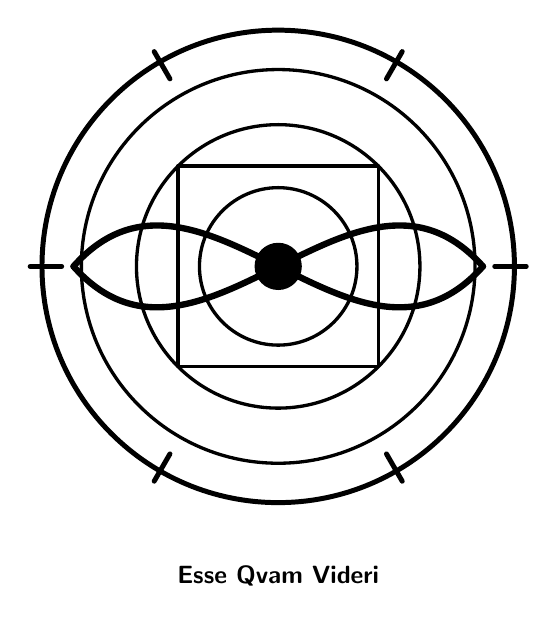
\begin{tikzpicture}[scale=1, line cap=round, line join=round]

\begin{scope}[xshift=7.5cm, yshift=-6.5cm]
  \draw[line width=1.8pt] (0,0) circle (3);
  \foreach \r in {1.0,1.8,2.5}
    \draw[line width=1.2pt] (0,0) circle (\r);
  \draw[line width=2.3pt]
    (-2.6,0) .. controls (-1.0,1.8) and (1.0,-1.8) .. (2.6,0);
  \draw[line width=2.3pt]
    (-2.6,0) .. controls (-1.0,-1.8) and (1.0,1.8) .. (2.6,0);
  \foreach \a in {0,60,120,180,240,300}
    \draw[line width=1.8pt] (\a:2.75) -- (\a:3.15);
  \draw[line width=1.3pt]
    (45:1.8)--(135:1.8)--(225:1.8)--(315:1.8)--cycle;
  \fill (0,0) circle (0.30);
  \node[below=8pt,font=\sffamily\bfseries\small] at (0,-3.4) {Esse Qvam Videri};
\end{scope}

\end{tikzpicture}

\end{document} 
